\documentclass{report}

\usepackage{graphicx}
\graphicspath{{./Apostol/images/}}

\usepackage{amsfonts, amsmath, amssymb, amsthm}
\usepackage{bigfoot}
\usepackage{comment}
\usepackage[shortlabels]{enumitem}
\usepackage{etoolbox}
\usepackage{environ}
\usepackage{fontawesome5}
\usepackage{mathabx, mathrsfs}
\usepackage{soul}
\usepackage{stmaryrd}
% Must load `xcolor` before `tcolorbox` and `tikz`.
\usepackage[dvipsnames]{xcolor}
\usepackage{tcolorbox}
\usepackage{tikz}
% `hyperref` comes after `xr-hyper`.
\usepackage{xr-hyper}
\usepackage{hyperref}

% Open "private" namespace.
\makeatletter

% ========================================
% General
% ========================================

\newcommand{\header}[2]{\title{#1}\author{#2}\date{}\maketitle}

% ========================================
% Dividers
% ========================================

\newcommand\@linespace{\vspace{10pt}}
\newcommand\linedivider{\@linespace\hrule\@linespace}
\WithSuffix\newcommand\linedivider*{\@linespace\hrule}
\newcommand\suitdivider{$$\spadesuit\;\spadesuit\;\spadesuit$$}

% ========================================
% Linking
% ========================================

\hypersetup{colorlinks=true, linkcolor=blue, urlcolor=blue}
\newcommand{\textref}[1]{\text{\nameref{#1}}}
\newcommand{\hyperlabel}[1]{%
  \label{#1}%
  \hypertarget{#1}{}}

% Links to theorems/statements/etc. that can be found in Mathlib4's index.
\newcommand\@leanlink[3]{%
  \textcolor{BlueViolet}{\raisebox{-4.5pt}{%
    \tikz{\draw (0, 0) node[yscale=-1,xscale=1] {\faFont};}}{-\;}}%
  \href{https://leanprover-community.github.io/mathlib4_docs/#1.html\##2}%
  {\color{BlueViolet}{#3}}}

\newcommand\lean[2]{%
  \noindent\@leanlink{#1}{#2}{#2}}
\WithSuffix\newcommand\lean*[2]{%
  \vspace{6pt}\lean{#1}{#2}}

\newcommand\leanp[3]{%
  \noindent\@leanlink{#1}{#2}{#3}}
\WithSuffix\newcommand\leanp*[3]{%
  \vspace{6pt}\leanp{#1}{#2}{#3}}

% Links to theorems/statements/etc. found in custom index.
\newcommand\@codelink[4]{%
  \textcolor{MidnightBlue}{\raisebox{-4.5pt}{%
    \tikz{\draw (0, 0) node[xshift=8pt] {\faCodeBranch};}}{-\;}}%
  \href{#1/#2.html\##3}%
  {\color{MidnightBlue}{#4}}}

\newcommand\coderef[3]{%
  \@codelink{#1}{#2}{#3}{#3}}
\newcommand\codepref[4]{%
  \@codelink{#1}{#2}{#3}{#4}}

% Macro to build our `code` commands relative to a given directory. For
% instance, we expect to have invocation `\makecode{..}` if the TeX file exists
% one directory deep from the root of our project..
\newcommand\makecode[1]{%
  \newcommand\code[2]{%
    \noindent\coderef{#1}{##1}{##2}}
  \WithSuffix\newcommand\code*[2]{%
    \vspace{6pt}\noindent\coderef{#1}{##1}{##2}}

  \newcommand\codep[3]{%
    \noindent\codepref{#1}{##1}{##2}{##3}}
  \WithSuffix\newcommand\codep*[3]{%
    \vspace{6pt}\noindent\codepref{#1}{##1}{##2}{##3}}
}

% ========================================
% Admonitions
% ========================================

\NewEnviron{note}{%
  \begin{tcolorbox}[%
      sharp corners,
      fonttitle=\sffamily\bfseries,
      toptitle=2pt,
      bottomtitle=2pt,
      coltitle=black!80!white,
      colback=yellow!30,
      colframe=yellow!80!black,
      title=Note]
    \BODY
  \end{tcolorbox}}

% ========================================
% Statements
% ========================================

\newcommand\@statement[1]{%
  \linedivider*\paragraph{\normalfont\normalsize\textit{#1.}}}
\newenvironment{answer}{\@statement{Answer}}{\hfill$\square$}
\renewenvironment{proof}{\@statement{Proof}}{\hfill$\square$}

\newtheorem{corollaryinner}{Corollary}
\newenvironment{corollary}[1][]{%
  \ifstrempty{#1}
    {\corollaryinner}
    {\renewcommand\thecorollaryinner{#1}\corollaryinner}
}{\endcorollaryinner}

\newtheorem{lemmainner}{Lemma}
\newenvironment{lemma}[1][]{%
  \ifstrempty{#1}
    {\lemmainner}
    {\renewcommand\thelemmainner{#1}\lemmainner}
}{\endlemmainner}

\newtheorem{theoreminner}{Theorem}
\newenvironment{theorem}[1][]{%
  \ifstrempty{#1}
    {\theoreminner}
    {\renewcommand\thetheoreminner{#1}\theoreminner}
}{\endtheoreminner}

% ========================================
% Status
% ========================================

\DeclareRobustCommand{\defined}[1]{%
  \texorpdfstring{\color{darkgray}\faParagraph\ #1}{#1}}
\DeclareRobustCommand{\verified}[1]{%
  \texorpdfstring{\color{teal}\faCheckCircle\ #1}{#1}}
\DeclareRobustCommand{\unverified}[1]{%
  \texorpdfstring{\color{olive}\faCheckCircle[regular]\ #1}{#1}}
\DeclareRobustCommand{\pending}[1]{%
  \texorpdfstring{\color{Fuchsia}\faPencil*\ #1}{#1}}
\DeclareRobustCommand{\sorry}[1]{%
  \texorpdfstring{\color{Maroon}\faExclamationCircle\ #1}{#1}}

% ========================================
% Math
% ========================================

\newcommand{\abs}[1]{\left|#1\right|}
\newcommand{\ceil}[1]{\left\lceil#1\right\rceil}
\newcommand{\dom}[1]{\textop{dom}{#1}}
\newcommand{\fld}[1]{\textop{fld}{#1}}
\newcommand{\floor}[1]{\left\lfloor#1\right\rfloor}
\newcommand{\icc}[2]{\left[#1, #2\right]}
\newcommand{\ico}[2]{\left[#1, #2\right)}
\newcommand{\img}[2]{#1\!\left\llbracket#2\right\rrbracket}
\newcommand{\ioc}[2]{\left(#1, #2\right]}
\newcommand{\ioo}[2]{\left(#1, #2\right)}
\newcommand{\powerset}[1]{\mathscr{P}#1}
\newcommand{\ran}[1]{\textop{ran}{#1}}
\newcommand{\textop}[1]{\mathop{\text{#1}}}
\newcommand{\ubar}[1]{\text{\b{$#1$}}}

\let\oldemptyset\emptyset
\let\emptyset\varnothing

% Close off "private" namespace.
\makeatother

\makeleancommands{..}

\begin{document}

\header
  {One-Variable Calculus, with an Introduction to Linear Algebra}
  {Tom M. Apostol}

\tableofcontents

\begingroup
\renewcommand\thechapter{R}
\setcounter{chapter}{0}
\addtocounter{chapter}{-1}

\chapter{Reference}%
\hyperlabel{chap:reference}

\section{\defined{Characteristic Function}}%
\hyperlabel{ref:characteristic-function}

  Let $S$ be a set of points on the real line.
  The \textbf{characteristic function} of $S$ is the function $\mathcal{X}_S$
    such that $\mathcal{X}_S(x) = 1$ for every $x$ in $S$, and
    $\mathcal{X}_S(x) = 0$ for those $x$ not in $S$.

  \code*{Common/Set/Basic}{Set.characteristic}

\section{\defined{Completeness Axiom}}%
\hyperlabel{ref:completeness-axiom}

  Every nonempty set $S$ of real numbers which is bounded above has a supremum;
    that is, there is a real number $B$ such that $B = \sup{S}$.

  \lean*{Mathlib/Data/Real/Basic}{Real.exists\_isLUB}

\section{\defined{Infimum}}%
\hyperlabel{ref:infimum}

  A number $B$ is called an \textbf{infimum} of a nonempty set $S$ if $B$ has
    the following two properties:
    \begin{enumerate}[(a)]
      \item $B$ is a lower bound for $S$.
      \item No number greater than $B$ is a lower bound for $S$.
    \end{enumerate}
  Such a number $B$ is also known as the \textbf{greatest lower bound}.

  \lean*{Mathlib/Order/Bounds/Basic}{IsGLB}

\section{\defined{Integrable}}%
\hyperlabel{ref:integrable}

  Let $f$ be a function defined and bounded on $[a, b]$.
  $f$ is said to be \textbf{integrable} if there exists one and only one number
    $I$ such that \eqref{ref:integral-bounded-function-eq2} holds.
  If $f$ is integrable on $[a, b]$, we say that the integral
    $\int_a^b f(x) \mathop{dx}$ \textbf{exists}.

\section{\defined{Integral of a Bounded Function}}%
\hyperlabel{ref:integral-bounded-function}

  Let $f$ be a function defined and bounded on $[a, b]$.
  Let $s$ and $t$ denote arbitrary step functions defined on $[a, b]$ such that
    \begin{equation}
      \hyperlabel{ref:integral-bounded-function-eq1}
      s(x) \leq f(x) \leq t(x)
    \end{equation}
    for every $x$ in $[a, b]$.
  If there is one and only one number $I$ such that
    \begin{equation}
      \hyperlabel{ref:integral-bounded-function-eq2}
      \int_a^b s(x) \mathop{dx} \leq I \leq \int_a^b t(x) \mathop{dx}
    \end{equation}
    for every pair of step functions $s$ and $t$ satisfying
    \eqref{ref:integral-bounded-function-eq1}, then this number $I$ is called
    the \textbf{integral of $f$ from $a$ to $b$}, and is denoted by the symbol
    $\int_a^b f(x) \mathop{dx}$ or by $\int_a^b f$.

  If $a < b$, we define
    $\int_b^a f(x) \mathop{dx} = -\int_a^b f(x) \mathop{dx}$,
    provided $f$ is \nameref{ref:integrable} on $[a, b]$.
  We also define $\int_a^a f(x) \mathop{dx} = 0$.

  The function $f$ is called the \textbf{integrand}, the numbers $a$ and $b$ are
    called the \textbf{limits of integration}, and the interval $[a, b]$ the
    \textbf{interval of integration}.

\section{\defined{Integral of a Step Function}}%
\hyperlabel{ref:integral-step-function}

  Let $s$ be a \nameref{ref:step-function} defined on $[a, b]$, and let
    $P = \{x_0, x_1, \ldots, x_n\}$ be a \nameref{ref:partition} of $[a, b]$
    such that $s$ is constant on the open subintervals of $P$.
  Denote by $s_k$ the constant value that $s$ takes in the $k$th open
    subinterval of $P$, so that
    $$s(x) = s_k \quad\text{if}\quad x_{k-1} < x < x_k, \quad k
           = 1, 2, \ldots, n.$$
  The \textbf{integral of $s$ from $a$ to $b$}, denoted by the symbol
    $\int_a^b s(x)\mathop{dx}$, is defined by the following formula:
    $$\int_a^b s(x) \mathop{dx} = \sum_{k=1}^n s_k \cdot (x_k - x_{k-1}).$$
  If $a < b$, we define
    $\int_b^a s(x) \mathop{dx} = -\int_a^b s(x) \mathop{dx}$.
  We also define $\int_a^a s(x) \mathop{dx} = 0$.

\section{\defined{Lower Integral}}%
\hyperlabel{ref:lower-integral}

  Let $f$ be a function bounded on $[a, b]$ and $S$ denote the set of numbers
    $\int_a^b s(x) \mathop{dx}$ obtained as $s$ runs through all
    \nameref{ref:step-function}s below $f$.
  That is, let $$S = \left\{ \int_a^b s(x) \mathop{dx} : s \leq f \right\}.$$
  The number $\sup{S}$ is called the \textbf{lower integral of $f$}.
  It is denoted as $\ubar{I}(f)$.

\section{\defined{Monotonic}}%
\hyperlabel{ref:monotonic}

  A function $f$ is called \textbf{monotonic} on set $S$ if it is increasing on
    $S$ or if it is decreasing on $S$.
  $f$ is said to be \textbf{strictly monotonic} if it is strictly increasing on
    $S$ or strictly decreasing on $S$.

  A function $f$ is said to be \textbf{piecewise monotonic} on an interval if
    its graph consists of a finite number of monotonic pieces.
  In other words, $f$ is piecewise monotonic on $[a, b]$ if there is a
    \nameref{ref:partition} of $[a, b]$ such that $f$ is monotonic on each of
    the open subintervals of $P$.

\section{\defined{Partition}}%
\hyperlabel{ref:partition}

  Let $[a, b]$ be a closed interval decomposed into $n$ subintervals by
    inserting $n - 1$ points of subdivision, say $x_1$, $x_2$, $\ldots$,
    $x_{n-1}$, subject only to the restriction
    \begin{equation}
      \hyperlabel{sec:partition-eq1}
      a < x_1 < x_2 < \cdots < x_{n-1} < b.
    \end{equation}
  It is convenient to denote the point $a$ itself by $x_0$ and the point $b$ by
    $x_n$.
  A collection of points satisfying \eqref{sec:partition-eq1} is called a
    \textbf{partition} $P$ of $[a, b]$, and we use the symbol
    $$P = \{x_0, x_1, \ldots, x_n\}$$ to designate this partition.

  \code*{Common/Set/Partition}{Set.Partition}

\section{\defined{Refinement}}%
\hyperlabel{ref:refinement}

  Let $P$ be a \nameref{ref:partition} of closed interval $[a, b]$.
  A \textbf{refinement} $P'$ of $P$ is a partition formed by adjoining more
    subdivision points to those already in $P$.

  $P'$ is said to be \textbf{finer than} $P$. The union of two partitions $P_1$
    and $P_2$ is called the \textbf{common refinement} of $P_1$ and $P_2$.

\section{\defined{Step Function}}%
\hyperlabel{ref:step-function}

  A function $s$, whose domain is a closed interval $[a, b]$, is called a
    \textbf{step function} if there is a \nameref{ref:partition}
    $P = \{x_0, x_1, \ldots, x_n\}$ of $[a, b]$ such that $s$ is constant on each
    open subinterval of $P$.
  That is to say, for each $k = 1, 2, \ldots, n$, there is a real number $s_k$
    such that $$s(x) = s_k \quad\text{if}\quad x_{k-1} < x < x_k.$$
    Step functions are sometimes called \textbf{piecewise constant functions}.

  \begin{note}
    At each of the endpoints $x_{k-1}$ and $x_k$ the function must have some
      well-defined value, but this need not be the same as $s_k$.
  \end{note}

  \code{Common/Geometry/StepFunction}{Geometry.StepFunction}

\section{\defined{Supremum}}%
\hyperlabel{ref:supremum}

  A number $B$ is called a \textbf{supremum} of a nonempty set $S$ if $B$ has
    the following two properties:
    \begin{enumerate}[(a)]
      \item $B$ is an upper bound for $S$.
      \item No number less than $B$ is an upper bound for $S$.
    \end{enumerate}
  Such a number $B$ is also known as the \textbf{least upper bound}.

  \lean*{Mathlib/Order/Bounds/Basic}{IsLUB}

\section{\defined{Upper Integral}}%
\hyperlabel{ref:upper-integral}

  Let $f$ be a function bounded on $[a, b]$ and $T$ denote the set of numbers
    $\int_a^b t(x) \mathop{dx}$ obtained as $t$ runs through all
    \nameref{ref:step-function}s above $f$.
  That is, let $$T = \left\{ \int_a^b t(x) \mathop{dx} : f \leq t \right\}.$$
  The number $\inf{T}$ is called the \textbf{upper integral of $f$}.
  It is denoted as $\bar{I}(f)$.

\endgroup

\chapter{A Set of Axioms for the Real-Number System}%
\hyperlabel{chap:set-axioms-real-number-system}

\section{\verified{Lemma 1}}%
\hyperlabel{sec:lemma-1}

  \begin{lemma}[1]
    Nonempty set $S$ has supremum $L$ if and only if set $-S$ has infimum $-L$.
  \end{lemma}

  \code{Bookshelf/Apostol/Chapter\_I\_03}
    {Apostol.Chapter\_I\_03.is\_lub\_neg\_set\_iff\_is\_glb\_set\_neg}

  \begin{proof}
    Suppose $L = \sup{S}$ and fix $x \in S$.
    By definition of the \nameref{ref:supremum}, $x \leq L$ and $L$ is the
      smallest value satisfying this inequality.
    Negating both sides of the inequality yields $-x \geq -L$.
    Furthermore, $-L$ must be the largest value satisfying this inequality.
    Therefore $-L = \inf{-S}$.
  \end{proof}

\section{\verified{Existence of a Greatest Lower Bound}}
\hyperlabel{sec:existence-greatest-lower-bound}
\hyperlabel{sec:theorem-i.27}

  \begin{theorem}[I.27]
    Every nonempty set $S$ that is bounded below has a greatest lower bound;
      that is, there is a real number $L$ such that $L = \inf{S}$.
  \end{theorem}

  \code{Bookshelf/Apostol/Chapter\_I\_03}
    {Apostol.Chapter\_I\_03.exists\_isGLB}

  \begin{proof}
    Let $S$ be a nonempty set bounded below by $x$.
    Then $-S$ is nonempty and bounded above by $x$.
    By the \nameref{ref:completeness-axiom}, there exists a
      \nameref{ref:supremum} $L$ of $-S$.
    By \nameref{sec:lemma-1}, $L$ is a supremum of $-S$ if and only if $-L$ is
      an infimum of $S$.
  \end{proof}

\section{\verified{Positive Integers Unbounded Above}}%
\hyperlabel{sec:positive-integers-unbounded-above}
\hyperlabel{sec:theorem-i.29}

  \begin{theorem}[I.29]
    For every real $x$ there exists a positive integer $n$ such that $n > x$.
  \end{theorem}

  \code{Bookshelf/Apostol/Chapter\_I\_03}
    {Apostol.Chapter\_I\_03.exists\_pnat\_geq\_self}

  \begin{proof}
    Let $n = \abs{\ceil{x}} + 1$.
    It is trivial to see $n$ is a positive integer satisfying $n \geq 1$.
    Thus all that remains to be shown is that $n > x$.
    If $x$ is nonpositive, $n > x$ immediately follows from $n \geq 1$.
    If $x$ is positive,
      $$x = \abs{x} \leq \abs{\ceil{x}} < \abs{\ceil{x}} + 1 = n.$$
  \end{proof}

\section{\verified{Archimedean Property of the Reals}}%
\hyperlabel{sec:archimedean-property-reals}
\hyperlabel{sec:theorem-i.30}

  \begin{theorem}[I.30]
    If $x > 0$ and if $y$ is an arbitrary real number, there exists a positive
      integer $n$ such that $nx > y$.
  \end{theorem}

  \code{Bookshelf/Apostol/Chapter\_I\_03}
    {Apostol.Chapter\_I\_03.exists\_pnat\_mul\_self\_geq\_of\_pos}

  \begin{proof}
    Let $x > 0$ and $y$ be an arbitrary real number.
    By \nameref{sec:theorem-i.29}, there exists a positive integer $n$ such that
      $n > y / x$.
    Multiplying both sides of the inequality yields $nx > y$ as expected.
  \end{proof}

\section{\verified{Theorem I.31}}%
\hyperlabel{sec:theorem-i.31}

  \begin{theorem}[I.31]
    If three real numbers $a$, $x$, and $y$ satisfy the inequalities
      $$a \leq x \leq a + \frac{y}{n}$$ for every integer $n \geq 1$, then
      $x = a$.
  \end{theorem}

  \code{Bookshelf/Apostol/Chapter\_I\_03}
    {Apostol.Chapter\_I\_03.forall\_pnat\_leq\_self\_leq\_frac\_imp\_eq}

  \begin{proof}

    By the trichotomy of the reals, there are three cases to consider:

    \paragraph{Case 1}%

      Suppose $x = a$.
      Then we are immediately finished.

    \paragraph{Case 2}%

      Suppose $x < a$.
      But by hypothesis, $a \leq x$.
      Thus $a < a$, a contradiction.

    \paragraph{Case 3}%

      Suppose $x > a$.
      Then there exists some $c > 0$ such that $a + c = x$.
      By \nameref{sec:archimedean-property-reals}, there exists an integer
        $n > 0$ such that $nc > y$.
      Rearranging terms, we see $y / n < c$.
      Therefore $a + y / n < a + c = x$.
      But by hypothesis, $x \leq a + y / n$.
      Thus $a + y / n < a + y / n$, a contradiction.

    \paragraph{Conclusion}%

      Since these cases are exhaustive and both case 2 and 3 lead to
        contradictions, $x = a$ is the only possibility.

  \end{proof}

\section{\verified{Lemma 2}}%
\hyperlabel{sec:lemma-2}

  \begin{lemma}[2]
    If three real numbers $a$, $x$, and $y$ satisfy the inequalities
      $$a - y / n \leq x \leq a$$ for every integer $n \geq 1$, then $x = a$.
  \end{lemma}

  \code{Bookshelf/Apostol/Chapter\_I\_03}
    {Apostol.Chapter\_I\_03.forall\_pnat\_frac\_leq\_self\_leq\_imp\_eq}

  \begin{proof}

    By the trichotomy of the reals, there are three cases to consider:

    \paragraph{Case 1}%

      Suppose $x = a$.
      Then we are immediately finished.

    \paragraph{Case 2}%

      Suppose $x < a$.
      Then there exists some $c > 0$ such that $x = a - c$.
      By \nameref{sec:archimedean-property-reals}, there exists an integer
        $n > 0$ such that $nc > y$.
      Rearranging terms, we see that $y / n < c$.
      Therefore $a - y / n > a - c = x$.
      But by hypothesis, $x \geq a - y / n$.
      Thus $a - y / n < a - y / n$, a contradiction.

    \paragraph{Case 3}%

      Suppose $x > a$.
      But by hypothesis $x \leq a$.
      Thus $a < a$, a contradiction.

    \paragraph{Conclusion}%

      Since these cases are exhaustive and both case 2 and 3 lead to
        contradictions, $x = a$ is the only possibility.

  \end{proof}

\section{\verified{Theorem I.32}}%
\hyperlabel{sec:theorem-i.32}

  Let $h$ be a given positive number and let $S$ be a set of real numbers.

\subsection{\verified{Theorem I.32a}}%
\hyperlabel{sub:theorem-i.32a}

  \begin{theorem}[I.32a]
    If $S$ has a supremum, then for some $x$ in $S$ we have $x > \sup{S} - h$.
  \end{theorem}

  \code{Bookshelf/Apostol/Chapter\_I\_03}
    {Apostol.Chapter\_I\_03.sup\_imp\_exists\_gt\_sup\_sub\_delta}

  \begin{proof}
    By definition of a \nameref{ref:supremum}, $\sup{S}$ is the least upper
      bound of $S$.
    For the sake of contradiction, suppose for all $x \in S$,
      $x \leq \sup{S} - h$.
    This immediately implies $\sup{S} - h$ is an upper bound of $S$.
    But $\sup{S} - h < \sup{S}$, contradicting $\sup{S}$ being the
      \textit{least} upper bound.
    Therefore our original hypothesis was wrong.
    That is, there exists some $x \in S$ such that $x > \sup{S} - h$.
  \end{proof}

\subsection{\verified{Theorem I.32b}}%
\hyperlabel{sub:theorem-i.32b}

  \begin{theorem}[I.32b]
    If $S$ has an infimum, then for some $x$ in $S$ we have $x < \inf{S} + h$.
  \end{theorem}

  \code{Bookshelf/Apostol/Chapter\_I\_03}
    {Apostol.Chapter\_I\_03.inf\_imp\_exists\_lt\_inf\_add\_delta}

  \begin{proof}
    By definition of an \nameref{ref:infimum}, $\inf{S}$ is the greatest lower
      bound of $S$.
    For the sake of contradiction, suppose for all $x \in S$,
      $x \geq \inf{S} + h$.
    This immediately implies $\inf{S} + h$ is a lower bound of $S$.
    But $\inf{S} + h > \inf{S}$, contradicting $\inf{S}$ being the
      \textit{greatest} lower bound.
    Therefore our original hypothesis was wrong.
    That is, there exists some $x \in S$ such that $x < \inf{S} + h$.
  \end{proof}

\section{\verified{Additive Property of Supremums and Infimums}}%
\hyperlabel{sec:additive-property-supremums-infimums}
\hyperlabel{sec:theorem-i.33}

  Given nonempty subsets $A$ and $B$ of $\mathbb{R}$, let $C$ denote the set
    $$C = \{a + b : a \in A, b \in B\}.$$

  \begin{note}
    This is known as the "Additive Property."
  \end{note}

\subsection{\verified{Theorem I.33a}}%
\hyperlabel{sub:theorem-i.33a}

  \begin{theorem}[I.33a]
    If each of $A$ and $B$ has a supremum, then $C$ has a supremum, and
      $$\sup{C} = \sup{A} + \sup{B}.$$
  \end{theorem}

  \code{Bookshelf/Apostol/Chapter\_I\_03}
    {Apostol.Chapter\_I\_03.sup\_minkowski\_sum\_eq\_sup\_add\_sup}

  \begin{proof}

    We prove (i) $\sup{A} + \sup{B}$ is an upper bound of $C$ and (ii)
      $\sup{A} + \sup{B}$ is the \textit{least} upper bound of $C$.

    \paragraph{(i)}%
    \hyperlabel{par:theorem-i.33a-i}

      Let $x \in C$.
      By definition of $C$, there exist elements $a' \in A$ and $b' \in B$ such
        that $x = a' + b'$.
      By definition of a \nameref{ref:supremum}, $a' \leq \sup{A}$.
      Likewise, $b' \leq \sup{B}$.
      Therefore $a' + b' \leq \sup{A} + \sup{B}$.
      Since $x = a' + b'$ was arbitrarily chosen, it follows $\sup{A} + \sup{B}$
        is an upper bound of $C$.

    \paragraph{(ii)}%

      Since $A$ and $B$ have supremums, $C$ is nonempty.
      By \nameref{par:theorem-i.33a-i}, $C$ is bounded above.
      Therefore the completeness axiom tells us $C$ has a supremum.
      Let $n > 0$ be an integer.
      We now prove that
        \begin{equation}
          \hyperlabel{par:theorem-i.33a-ii-eq1}
          \sup{C} \leq \sup{A} + \sup{B} \leq \sup{C} + 1 / n.
        \end{equation}

      \subparagraph{Left-Hand Side}%

        First consider the left-hand side of \eqref{par:theorem-i.33a-ii-eq1}.
        By \nameref{par:theorem-i.33a-i}, $\sup{A} + \sup{B}$ is an upper bound
          of $C$.
        Since $\sup{C}$ is the \textit{least} upper bound of $C$, it follows
          $\sup{C} \leq \sup{A} + \sup{B}$.

      \subparagraph{Right-Hand Side}%

        Next consider the right-hand side of \eqref{par:theorem-i.33a-ii-eq1}.
        By \nameref{sub:theorem-i.32a}, there exists some $a' \in A$ such that
          $\sup{A} < a' + 1 / (2n)$.
        Likewise, there exists some $b' \in B$ such that
          $\sup{B} < b' + 1 / (2n)$.
        Adding these two inequalities together shows
          \begin{align*}
            \sup{A} + \sup{B}
              & < a' + b' + 1 / n \\
              & \leq \sup{C} + 1 / n.
          \end{align*}

      \subparagraph{Conclusion}%

        Applying \nameref{sec:theorem-i.31} to \eqref{par:theorem-i.33a-ii-eq1}
          proves $\sup{C} = \sup{A} + \sup{B}$ as expected.

  \end{proof}

\subsection{\verified{Theorem I.33b}}%
\hyperlabel{sub:theorem-i.33b}

  \begin{theorem}[I.33b]
    If each of $A$ and $B$ has an infimum, then $C$ has an infimum, and
      $$\inf{C} = \inf{A} + \inf{B}.$$
  \end{theorem}

  \code{Bookshelf/Apostol/Chapter\_I\_03}
    {Apostol.Chapter\_I\_03.inf\_minkowski\_sum\_eq\_inf\_add\_inf}

  \begin{proof}

    We prove (i) $\inf{A} + \inf{B}$ is a lower bound of $C$ and (ii)
      $\inf{A} + \inf{B}$ is the \textit{greatest} lower bound of $C$.

    \paragraph{(i)}%
    \hyperlabel{par:theorem-i.33b-i}

      Let $x \in C$.
      By definition of $C$, there exist elements $a' \in A$ and $b' \in B$ such
        that $x = a' + b'$.
      By definition of an \nameref{ref:infimum}, $a' \geq \inf{A}$.
      Likewise, $b' \geq \inf{B}$.
      Therefore $a' + b' \geq \inf{A} + \inf{B}$.
      Since $x = a' + b'$ was arbitrarily chosen, it follows $\inf{A} + \inf{B}$
        is a lower bound of $C$.

    \paragraph{(ii)}%

      Since $A$ and $B$ have infimums, $C$ is nonempty.
      By \nameref{par:theorem-i.33b-i}, $C$ is bounded below.
      Therefore \nameref{sec:theorem-i.27} tells us $C$ has an infimum.
      Let $n > 0$ be an integer.
      We now prove that
        \begin{equation}
          \hyperlabel{par:theorem-i.33b-ii-eq1}
          \inf{C} - 1 / n \leq \inf{A} + \inf{B} \leq \inf{C}.
        \end{equation}

      \subparagraph{Right-Hand Side}%

        First consider the right-hand side of \eqref{par:theorem-i.33b-ii-eq1}.
        By \nameref{par:theorem-i.33b-i}, $\inf{A} + \inf{B}$ is a lower bound
          of $C$.
        Since $\inf{C}$ is the \textit{greatest} upper bound of $C$, it follows
          $\inf{C} \geq \inf{A} + \inf{B}$.

      \subparagraph{Left-Hand Side}%

        Next consider the left-hand side of \eqref{par:theorem-i.33b-ii-eq1}.
        By \nameref{sub:theorem-i.32b}, there exists some $a' \in A$ such that
          $\inf{A} > a' - 1 / (2n)$.
        Likewise, there exists some $b' \in B$ such that
          $\inf{B} > b' - 1 / (2n)$.
        Adding these two inequalities together shows
          \begin{align*}
            \inf{A} + \inf{B}
              & > a' + b' - 1 / n \\
              & \geq \inf{C} - 1 / n.
          \end{align*}

      \subparagraph{Conclusion}%

        Applying \nameref{sec:lemma-2} to \eqref{par:theorem-i.33b-ii-eq1}
          proves $\inf{C} = \inf{A} + \inf{B}$ as expected.

  \end{proof}

\section{\verified{Theorem I.34}}%
\hyperlabel{sec:theorem-i.34}

  \begin{theorem}[I.34]
    Given two nonempty subsets $S$ and $T$ of $\mathbb{R}$ such that
      $$s \leq t$$ for every $s$ in $S$ and every $t$ in $T$. Then $S$ has a
      supremum, and $T$ has an infimum, and they satisfy the inequality
      $$\sup{S} \leq \inf{T}.$$
  \end{theorem}

  \code{Bookshelf/Apostol/Chapter\_I\_03}
    {Apostol.Chapter\_I\_03.forall\_mem\_le\_forall\_mem\_imp\_sup\_le\_inf}

  \begin{proof}
    By hypothesis, $S$ and $T$ are nonempty sets.
    Let $s \in S$ and $t \in T$.
    Then $t$ is an upper bound of $S$ and $s$ is a lower bound of $T$.
    By the completeness axiom, $S$ has a supremum.
    By \nameref{sec:theorem-i.27}, $T$ has an infimum.
    All that remains is showing $\sup{S} \leq \inf{T}$.

    For the sake of contradiction, suppose $\sup{S} > \inf{T}$.
    Then there exists some $c > 0$ such that $\sup{S} = \inf{T} + c$.
    Therefore $\inf{T} < \sup{S} - c / 2$.
    By \nameref{sub:theorem-i.32a}, there exists some $x \in S$ such that
      $\sup{S} - c / 2 < x$.
    Thus $$\inf{T} < \sup{S} - c / 2 < x.$$
    But by hypothesis, $x \in S$ is a lower bound of $T$ meaning
      $x \leq \inf{T}$.
    Therefore $x < x$, a contradiction.
    Out original assumption is incorrect; that is, $\sup{S} \leq \inf{T}$.
  \end{proof}

\chapter{The Concepts of Integral Calculus}%
\hyperlabel{chap:concepts-integral-calculus}

\section{The Concept of Area as a Set Function}%
\hyperlabel{sec:concept-area-set-function}

  We assume there exists a class $\mathscr{M}$ of measurable sets in the plane and
    a set function $a$, whose domain is $\mathscr{M}$, with the following
    properties:

\subsection{\defined{Nonnegative Property}}%
\hyperlabel{sub:nonnegative-property}

  For each set $S$ in $\mathscr{M}$, we have $a(S) \geq 0$.

  \codep*{Common/Geometry/Area}{Nonnegative-Property}
    {Nonnegative Property}

\subsection{\defined{Additive Property}}%
\hyperlabel{sub:area-additive-property}

  If $S$ and $T$ are in $\mathscr{M}$, then $S \cup T$ and $S \cap T$ are in
    $\mathscr{M}$, and we have $a(S \cup T) = a(S) + a(T) - a(S \cap T)$.

  \codep*{Common/Geometry/Area}{Additive-Property}
    {Additive Property}

\subsection{\defined{Difference Property}}%
\hyperlabel{sub:area-difference-property}

  If $S$ and $T$ are in $\mathscr{M}$ with $S \subseteq T$, then $T - S$ is in
    $\mathscr{M}$, and we have $a(T - S) = a(T) - a(S)$.

  \codep*{Common/Geometry/Area}{Difference-Property}
    {Difference Property}

\subsection{\defined{Invariance Under Congruence}}%
\hyperlabel{sub:area-invariance-under-congruence}

  If a set $S$ is in $\mathscr{M}$ and if $T$ is congruent to $S$, then $T$ is
    also in $\mathscr{M}$ and we have $a(S) = a(T)$.

  \codep*{Common/Geometry/Area}{Invariance-Under-Congruence}
    {Invariance Under Congruence}

\subsection{\defined{Choice of Scale}}%
\hyperlabel{sub:area-choice-scale}

  Every rectangle $R$ is in $\mathscr{M}$.
  If the edges of $R$ have lengths $h$ and $k$, then $a(R) = hk$.

  \codep*{Common/Geometry/Area}{Choice-of-Scale}
    {Choice of Scale}

\subsection{\pending{Exhaustion Property}}%
\hyperlabel{sub:area-exhaustion-property}

  Let $Q$ be a set that can be enclosed between two step regions $S$ and $T$, so
    that
    \begin{equation}
      \hyperlabel{sub:exhaustion-property-eq1}
      S \subseteq Q \subseteq T.
    \end{equation}
  If there is one and only one number $c$ which satisfies the inequalities
    $$a(S) \leq c \leq a(T)$$ for all step regions $S$ and $T$ satisfying
    \eqref{sub:exhaustion-property-eq1}, then $Q$ is measurable and $a(Q) = c$.

  \codep*{Common/Geometry/Area}{Exhaustion-Property}
    {Exhaustion Property}

\section{Exercises 1.7}%
\hyperlabel{sec:exercises-1.7}

\subsection{\pending{Exercise 1.7.1}}%
\hyperlabel{sub:exercise-1.7.1}

  Prove that each of the following sets is measurable and has zero area:

\subsubsection{\pending{Exercise 1.7.1a}}%
\hyperlabel{ssub:exercise-1.7.1a}

  A set consisting of a single point.

  \begin{proof}
    Let $S$ be a set consisting of a single point.
    By definition of a point, $S$ is a rectangle in which all vertices coincide.
    By \nameref{sub:area-choice-scale}, $S$ is measurable with area its width
      times its height.
    The width and height of $S$ is trivially zero.
    Therefore $a(S) = (0)(0) = 0$.
  \end{proof}

\subsubsection{\pending{Exercise 1.7.1b}}%
\hyperlabel{ssub:exercise-1.7.1b}

  A set consisting of a finite number of points in a plane.

  \begin{proof}

    Define predicate $P(n)$ as "A set consisting of $n$ points in a plane is
      measurable with area $0$".
    We use induction to prove $P(n)$ holds for all $n > 0$.

    \paragraph{Base Case}%

      Consider a set $S$ consisting of a single point in a plane.
      By \nameref{ssub:exercise-1.7.1a}, $S$ is measurable with area $0$.
      Thus $P(1)$ holds.

    \paragraph{Induction Step}%

      Assume induction hypothesis $P(k)$ holds for some $k > 0$.
      Let $S_{k+1}$ be a set consisting of $k + 1$ points in a plane.
      Pick an arbitrary point of $S_{k+1}$.
      Denote the set containing just this point as $T$.
      Denote the remaining set of points as $S_k$.
      By construction, $S_{k+1} = S_k \cup T$.
      By the induction hypothesis, $S_k$ is measurable with area $0$.
      By \nameref{ssub:exercise-1.7.1a}, $T$ is measurable with area $0$.
      By the \nameref{sub:area-additive-property}, $S_k \cup T$ is
        measurable, $S_k \cap T$ is measurable, and
        \begin{align}
          a(S_{k+1})
            & = a(S_k \cup T) \nonumber \\
            & = a(S_k) + a(T) - a(S_k \cap T) \nonumber \\
            & = 0 + 0 - a(S_k \cap T). \hyperlabel{ssub:exercise-1.7.1b-eq1}
        \end{align}
      There are two cases to consider:

      \subparagraph{Case 1}%

        $S_k \cap T = \emptyset$.
        Then it trivially follows that $a(S_k \cap T) = 0$.

      \subparagraph{Case 2}%

        $S_k \cap T \neq \emptyset$.
        Since $T$ consists of a single point, $S_k \cap T = T$.
        By \nameref{ssub:exercise-1.7.1a}, $a(S_k \cap T) = a(T) = 0$.

      \vspace{8pt}
      \noindent
      In both cases, \eqref{ssub:exercise-1.7.1b-eq1} evaluates to $0$, implying
        $P(k + 1)$ as expected.

    \paragraph{Conclusion}%

      By mathematical induction, it follows for all $n > 0$, $P(n)$ is true.

  \end{proof}

\subsubsection{\pending{Exercise 1.7.1c}}%
\hyperlabel{ssub:exercise-1.7.1c}

The union of a finite collection of line segments in a plane.

\begin{proof}

  Define predicate $P(n)$ as "A set consisting of $n$ line segments in a plane
    is measurable with area $0$".
  We use induction to prove $P(n)$ holds for all $n > 0$.

  \paragraph{Base Case}%

    Consider a set $S$ consisting of a single line segment in a plane.
    By definition of a line segment, $S$ is a rectangle in which one side has
      dimension $0$.
    By \nameref{sub:area-choice-scale}, $S$ is measurable with area its width
      $w$ times its height $h$.
    Therefore $a(S) = wh = 0$.
    Thus $P(1)$ holds.

  \paragraph{Induction Step}%

    Assume induction hypothesis $P(k)$ holds for some $k > 0$.
    Let $S_{k+1}$ be a set consisting of $k + 1$ line segments in a plane.
    Pick an arbitrary line segment of $S_{k+1}$.
    Denote the set containing just this line segment as $T$.
    Denote the remaining set of line segments as $S_k$.
    By construction, $S_{k+1} = S_k \cup T$.
    By the induction hypothesis, $S_k$ is measurable with area $0$.
    By the base case, $T$ is measurable with area $0$.
    By the \nameref{sub:area-additive-property}, $S_k \cup T$ is measurable,
      $S_k \cap T$ is measurable, and
      \begin{align}
        a(S_{k+1})
          & = a(S_k \cup T) \nonumber \\
          & = a(S_k) + a(T) - a(S_k \cap T) \nonumber \\
          & = 0 + 0 - a(S_k \cap T). \hyperlabel{ssub:exercise-1.7.1c-eq1}
      \end{align}
    There are two cases to consider:

    \subparagraph{Case 1}%

      $S_k \cap T = \emptyset$.
      Then it trivially follows that $a(S_k \cap T) = 0$.

    \subparagraph{Case 2}%

      $S_k \cap T \neq \emptyset$.
      Since $T$ consists of a single point, $S_k \cap T = T$.
      By the base case, $a(S_k \cap T) = a(T) = 0$.

    \vspace{8pt}
    \noindent
    In both cases, \eqref{ssub:exercise-1.7.1c-eq1} evaluates to $0$, implying
      $P(k + 1)$ as expected.

  \paragraph{Conclusion}%

    By mathematical induction, it follows for all $n > 0$, $P(n)$ is true.

\end{proof}

\subsection{\pending{Exercise 1.7.2}}%
\hyperlabel{sub:exercise-1.7.2}

  Every right triangular region is measurable because it can be obtained as the
    intersection of two rectangles.
  Prove that every triangular region is measurable and that its area is one half
    the product of its base and altitude.

  \begin{proof}
    Let $T'$ be a triangular region with base of length $a$, height of length
      $b$, and hypotenuse of length $c$.
    Consider the translation and rotation of $T'$, say $T$, such that its
      hypotenuse is entirely within quadrant I and the vertex opposite the
      hypotenuse is situated at point $(0, 0)$.

    Let $R$ be a rectangle of width $a$, height $b$, and bottom-left corner at
      $(0, 0)$.
    By construction, $R$ covers all of $T$.
    Let $S$ be a rectangle of width $c$ and height $a\sin{\theta}$, where
      $\theta$ is the acute angle measured from the bottom-right corner of $T$
      relative to the $x$-axis.
    As an example, consider the image below of triangle $T$ with width $4$ and
      height $3$:

    \begin{figure}[ht]
      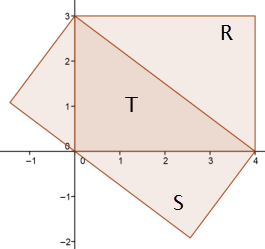
\includegraphics{right-triangle}
      \centering
    \end{figure}

    By \nameref{sub:area-choice-scale}, both $R$ and $S$ are measurable.
    By this same axiom, $a(R) = ab$ and $a(S) = ca\sin{\theta}$.
    By the \nameref{sub:area-additive-property}, $R \cup S$ and $R \cap S$ are
      both measurable.
    $a(R \cap S) = a(T)$ and $a(R \cup S)$ can be determined by noting that
      $R$'s construction implies identity $a(R) = 2a(T)$.
    Therefore
      \begin{align*}
        a(T)
          & = a(R \cap S) \\
          & = a(R) + a(S) - a(R \cup S) \\
          & = ab + ca\sin{\theta} - a(R \cup S) \\
          & = ab + ca\sin{\theta} - (ca\sin{\theta} + \frac{1}{2}a(R)) \\
          & = ab + ca\sin{\theta} - ca\sin{\theta} - a(T).
      \end{align*}
    Solving for $a(T)$ gives the desired identity: $$a(T) = \frac{1}{2}ab.$$
    By \nameref{sub:area-invariance-under-congruence}, $a(T') = a(T)$,
      concluding our proof.
  \end{proof}

\subsection{\pending{Exercise 1.7.3}}%
\hyperlabel{sub:exercise-1.7.3}

  Prove that every trapezoid and every parallelogram is measurable and derive
    the usual formulas for their areas.

  \begin{proof}

    We begin by proving the formula for a trapezoid.
    Let $S$ be a trapezoid with height $h$ and bases $b_1$ and $b_2$,
      $b_1 < b_2$.
    There are three cases to consider:

    \begin{figure}[ht]
      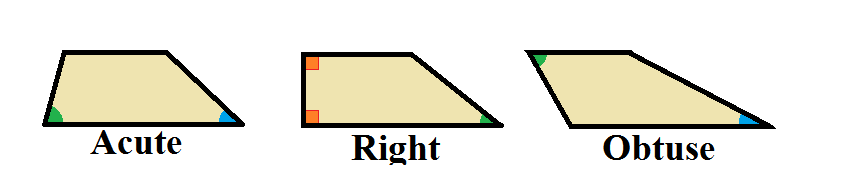
\includegraphics[width=\textwidth]{trapezoid-cases}
      \centering
    \end{figure}

    \paragraph{Case 1}%

      Suppose $S$ is a right trapezoid.
      Then $S$ is the union of non-overlapping rectangle $R$ of width $b_1$ and
        height $h$ with right triangle $T$ of base $b_2 - b_1$ and height $h$.
      By \nameref{sub:area-choice-scale}, $R$ is measurable.
      By \nameref{sub:exercise-1.7.2}, $T$ is measurable.
      By the \nameref{sub:area-additive-property}, $R \cup T$ and $R \cap T$ are
        both measurable and
        \begin{align*}
          a(S)
            & = a(R \cup T) \\
            & = a(R) + a(T) - a(R \cap T) \\
            & = a(R) + a(T) & \text{by construction} \\
            & = b_1h + a(T) & \text{Choice of Scale} \\
            & = b_1h + \frac{1}{2}(b_2 - b_1)h & \textref{sub:exercise-1.7.2} \\
            & = \frac{b_1 + b_2}{2}h.
        \end{align*}

    \paragraph{Case 2}%

      Suppose $S$ is an acute trapezoid.
      Then $S$ is the union of non-overlapping triangle $T$ and right trapezoid
        $R$.
      Let $c$ denote the length of base $T$.
      Then $R$ has longer base edge of length $b_2 - c$.
      By \nameref{sub:exercise-1.7.2}, $T$ is measurable.
      By Case 1, $R$ is measurable.
      By the \nameref{sub:area-additive-property}, $R \cup T$ and $R \cap T$ are
        both measurable and
        \begin{align*}
          a(S)
            & = a(T) + a(R) - a(R \cap T) \\
            & = a(T) + a(R) & \text{by construction} \\
            & = \frac{1}{2}ch + a(R) & \textref{sub:exercise-1.7.2} \\
            & = \frac{1}{2}ch + \frac{b_1 + b_2 - c}{2}h & \text{Case 1} \\
            & = \frac{b_1 + b_2}{2}h.
        \end{align*}

    \paragraph{Case 3}%

      Suppose $S$ is an obtuse trapezoid.
      Then $S$ is the union of non-overlapping triangle $T$ and right trapezoid
        $R$.
      Let $c$ denote the length of base $T$.
      Reflect $T$ vertically to form another right triangle, say $T'$.
      Then $T' \cup R$ is an acute trapezoid.
      By \nameref{sub:area-invariance-under-congruence},
        \begin{equation}
          \hyperlabel{sub:exercise-1.7.3-eq1}
          \tag{3.1}
          a(T' \cup R) = a(T \cup R).
        \end{equation}
      By construction, $T' \cup R$ has height $h$ and bases $b_1 - c$ and
        $b_2 + c$ meaning
        \begin{align*}
          a(T \cup R)
            & = a(T' \cup R) & \eqref{sub:exercise-1.7.3-eq1} \\
            & = \frac{b_1 - c + b_2 + c}{2}h & \text{Case 2} \\
            & = \frac{b_1 + b_2}{2}h.
        \end{align*}

    \paragraph{Conclusion}%

      These cases are exhaustive and in agreement with one another.
      Thus $S$ is measurable and $$a(S) = \frac{b_1 + b_2}{2}h.$$

    \suitdivider

    Let $P$ be a parallelogram with base $b$ and height $h$.
    Then $P$ is the union of non-overlapping triangle $T$ and right trapezoid
      $R$.
    Let $c$ denote the length of base $T$.
    Reflect $T$ vertically to form another right triangle, say $T'$.
    Then $T' \cup R$ is an acute trapezoid.
    By \nameref{sub:area-invariance-under-congruence},
      \begin{equation}
        \hyperlabel{sub:exercise-1.7.3-eq2}
        a(T' \cup R) = a(T \cup R).
      \end{equation}
    By construction, $T' \cup R$ has height $h$ and bases $b - c$ and $b + c$
      meaning
      \begin{align*}
        a(T \cup R)
          & = a(T' \cup R) & \eqref{sub:exercise-1.7.3-eq2} \\
          & = \frac{b - c + b + c}{2}h & \text{Area of Trapezoid} \\
          & = bh.
      \end{align*}

  \end{proof}

\subsection{\pending{Exercise 1.7.4}}%
\hyperlabel{sub:exercise-1.7.4}

  Let $P$ be a polygon whose vertices are lattice points.
  The area of $P$ is $I + \frac{1}{2}B - 1$, where $I$ denotes the number of
    lattice points inside the polygon and $B$ denotes the number on the
    boundary.

\subsubsection{\pending{Exercise 1.7.4a}}%
\hyperlabel{ssub:exercise-1.7.4a}

  Prove that the formula is valid for rectangles with sides parallel to the
    coordinate axes.

  \begin{proof}
    Let $P$ be a rectangle with sides parallel to the coordinate axes, with
      width $w$, height $h$, and lattice points for vertices.
    We assume $P$ has three non-collinear points, ruling out any instances of
      points or line segments.

    By \nameref{sub:area-choice-scale}, $P$ is measurable with area $a(P) = wh$.
    By construction, $P$ has $I = (w - 1)(h - 1)$ interior lattice points and
      $B = 2(w + h)$ lattice points on its boundary.
    The following shows the lattice point area formula is in agreement with
      the expected result:
      \begin{align*}
        I + \frac{1}{2}B - 1
          & = (w - 1)(h - 1) + \frac{1}{2}\left[ 2(w + h) \right] - 1 \\
          & = (wh - w - h + 1) + \frac{1}{2}\left[ 2(w + h) \right] - 1 \\
          & = (wh - w - h + 1) + (w + h) - 1 \\
          & = wh.
      \end{align*}
  \end{proof}

\subsubsection{\pending{Exercise 1.7.4b}}%
\hyperlabel{ssub:exercise-1.7.4b}

  Prove that the formula is valid for right triangles and parallelograms.

  \begin{proof}
    Let $P$ be a right triangle with width $w > 0$, height $h > 0$, and lattice
      points for vertices.
    Let $T$ be the triangle $P$ translated, rotated, and reflected such that the
      its vertices are $(0, 0)$, $(0, w)$, and $(w, h)$.
    Let $I_T$ and $B_T$ be the number of interior and boundary points of $T$
      respectively.
    Let $H_L$ denote the number of lattice points on $T$'s hypotenuse.

    Let $R$ be the overlapping rectangle of width $w$ and height $h$, situated
      with bottom-left corner at $(0, 0)$.
    Let $I_R$ and $B_R$ be the number of interior and boundary points
      of $R$ respectively.

    By construction, $T$ shares two sides with $R$.
    Therefore
      \begin{equation}
        \hyperlabel{ssub:exercise-1.7.4b-eq1}
        B_T = \frac{1}{2}B_R - 1 + H_L.
      \end{equation}
    Likewise,
      \begin{equation}
        \hyperlabel{ssub:exercise-1.7.4b-eq2}
        I_T = \frac{1}{2}(I_R - (H_L - 2)).
      \end{equation}
    The following shows the lattice point area formula is in agreement with
      the expected result:
      \begin{align*}
        I_T + \frac{1}{2}B_T - 1
          & = \frac{1}{2}(I_R - (H_L - 2)) + \frac{1}{2}B_T - 1
            & \eqref{ssub:exercise-1.7.4b-eq2} \\
          & = \frac{1}{2}\left[ I_R - H_L + B_T \right] \\
          & = \frac{1}{2}\left[ I_R - H_L + \frac{1}{2}B_R - 1 + H_L \right]
            & \eqref{ssub:exercise-1.7.4b-eq1} \\
          & = \frac{1}{2}\left[ I_R + \frac{1}{2}B_R - 1 \right] \\
          & = \frac{1}{2}\left[ wh \right] & \textref{ssub:exercise-1.7.4a}.
      \end{align*}

    We do not prove this formula is valid for parallelograms here.
    Instead, refer to \nameref{ssub:exercise-1.7.4c} below.
  \end{proof}

\subsubsection{\pending{Exercise 1.7.4c}}%
\hyperlabel{ssub:exercise-1.7.4c}

  Use induction on the number of edges to construct a proof for general
    polygons.

  \begin{proof}

    Define predicate $P(n)$ as "An $n$-polygon with vertices on lattice points
      has area $I + \frac{1}{2}B - 1$."
    We use induction to prove $P(n)$ holds for all $n \geq 3$.

    \paragraph{Base Case}%

      A $3$-polygon is a triangle.
      By \nameref{ssub:exercise-1.7.4b}, the lattice point area formula holds.
      Thus $P(3)$ holds.

    \paragraph{Induction Step}%

      Assume induction hypothesis $P(k)$ holds for some $k \geq 3$.
      Let $P$ be a $(k + 1)$-polygon with vertices on lattice points.
      Such a polygon is equivalent to the union of a $k$-polygon $S$ with a
        triangle $T$.
      That is, $P = S \cup T$.

      Let $I_P$ be the number of interior lattice points of $P$.
      Let $B_P$ be the number of boundary lattice points of $P$.
      Similarly, let $I_S$, $I_T$, $B_S$, and $B_T$ be the number of interior
        and boundary lattice points of $S$ and $T$.
      Let $c$ denote the number of boundary points shared between $S$ and $T$.

      By our induction hypothesis, $a(S) = I_S + \frac{1}{2}B_S - 1$.
      By our base case, $a(T) = I_T + \frac{1}{2}B_T - 1$.
      By construction, it follows:
        \begin{align*}
          I_P & = I_S + I_T + c - 2 \\
          B_P & = B_S + B_T - (c - 2) - c \\
              & = B_S + B_T - 2c + 2.
        \end{align*}
      Applying the lattice point area formula to $P$ yields the following:
        \begin{align*}
          & I_P + \frac{1}{2}B_P - 1 \\
            & = (I_S + I_T + c - 2) + \frac{1}{2}(B_S + B_T - 2c + 2) - 1 \\
            & = I_S + I_T + c - 2 + \frac{1}{2}B_S + \frac{1}{2}B_T - c + 1 - 1 \\
            & = (I_S + \frac{1}{2}B_S - 1) + (I_T + \frac{1}{2}B_T - 1) \\
            & = a(S) + (I_T + \frac{1}{2}B_T - 1) & \text{induction hypothesis} \\
            & = a(S) + a(T). & \text{base case}
        \end{align*}
      By the \nameref{sub:area-additive-property}, $S \cup T$ is measurable,
        $S \cap T$ is measurable, and
        \begin{align*}
          a(P)
            & = a(S \cup T) \\
            & = a(S) + a(T) - a(S \cap T) \\
            & = a(S) + a(T). & \text{by construction}
        \end{align*}
      This shows the lattice point area formula is in agreement with our
        axiomatic definition of area.
      Thus $P(k + 1)$ holds.

    \paragraph{Conclusion}%

      By mathematical induction, it follows for all $n \geq 3$, $P(n)$ is true.

  \end{proof}

\subsection{\pending{Exercise 1.7.5}}%
\hyperlabel{sub:exercise-1.7.5}

  Prove that a triangle whose vertices are lattice points cannot be equilateral.

  [\textit{Hint:} Assume there is such a triangle and compute its area in two
  ways, using Exercises 2 and 4.]

  \begin{proof}
    Proceed by contradiction.
    Let $T$ be an equilateral triangle whose vertices are lattice points.
    Assume each side of $T$ has length $a$.
    Then $T$ has height $h = (a\sqrt{3}) / 2$.
    By \nameref{sub:exercise-1.7.2},
      \begin{equation}
        \hyperlabel{sub:exercise-1.7.5-eq1}
        \tag{5.1}
        a(T) = \frac{1}{2}ah = \frac{a^2\sqrt{3}}{4}.
      \end{equation}
    Let $I$ and $B$ denote the number of interior and boundary lattice points of
      $T$ respectively.
    By \nameref{sub:exercise-1.7.4},
      \begin{equation}
        \hyperlabel{sub:exercise-1.7.5-eq2}
        \tag{5.2}
        a(T) = I + \frac{1}{2}B - 1.
      \end{equation}
    But \eqref{sub:exercise-1.7.5-eq1} is irrational whereas
      \eqref{sub:exercise-1.7.5-eq2} is not.
    This is a contradiction.
    Thus, there is \textit{no} equilateral triangle whose vertices are lattice
      points.
  \end{proof}

\subsection{\pending{Exercise 1.7.6}}%
\hyperlabel{sub:exercise-1.7.6}

  Let $A = \{1, 2, 3, 4, 5\}$, and let $\mathscr{M}$ denote the class of all
    subsets of $A$.
  (There are 32 altogether, counting $A$ itself and the empty set $\emptyset$.)
  For each set $S$ in $\mathscr{M}$, let $n(S)$ denote the number of distinct
    elements in $S$.
  If $S = \{1, 2, 3, 4\}$ and $T = \{3, 4, 5\}$, compute $n(S \cup T)$,
    $n(S \cap T)$, $n(S - T)$, and $n(T - S)$.
  Prove that the set function $n$ satisfies the first three axioms for area.

  \begin{proof}

    Let $S = \{1, 2, 3, 4\}$ and $T = \{3, 4, 5\}$.
    Then
      \begin{align*}
        n(S \cup T)
          & = n(\{1, 2, 3, 4\} \cup \{3, 4, 5\}) \\
          & = n(\{1, 2, 3, 4, 5\}) \\
          & = 5. \\
        n(S \cap T)
          & = n(\{1, 2, 3, 4\} \cap \{3, 4, 5\}) \\
          & = n(\{3, 4\}) \\
          & = 2. \\
        n(S - T)
          & = n(\{1, 2, 3, 4\} - \{3, 4, 5\}) \\
          & = n(\{1, 2\}) \\
          & = 2. \\
        n(T - S)
          & = n(\{3, 4, 5\} - \{1, 2, 3, 4\}) \\
          & = n(\{5\}) \\
          & = 1.
      \end{align*}
    We now prove $n$ satisfies the first three axioms for area.

    \paragraph{Nonnegative Property}%

      $n$ returns the length of some member of $\mathscr{M}$.
      By hypothesis, the smallest possible input to $n$ is $\emptyset$.
      Since $n(\emptyset) = 0$, it follows $n(S) \geq 0$ for all $S \subset A$.

    \paragraph{Additive Property}%

      Let $S$ and $T$ be members of $\mathscr{M}$.
      It trivially follows that both $S \cup T$ and $S \cap T$ are in
        $\mathscr{M}$.
      Consider the value of $n(S \cup T)$.
      There are two cases to consider:

      \subparagraph{Case 1}%

        Suppose $S \cap T = \emptyset$.
        That is, there is no common element shared between $S$ and $T$.
        Thus
          \begin{align*}
            n(S \cup T)
              & = n(S) + n(T) \\
              & = n(S) + n(T) - 0 \\
              & = n(S) + n(T) - n(S \cap T).
          \end{align*}

      \subparagraph{Case 2}%

        Suppose $S \cap T \neq \emptyset$.
        Then $n(S) + n(T)$ counts each element of $S \cap T$ twice.
        Therefore $n(S \cup T) = n(S) + n(T) - n(S \cap T)$.

      \subparagraph{Conclusion}%

        These cases are exhaustive and in agreement with one another.
        Thus $n(S \cup T) = n(S) + n(T) - n(S \cap T)$.

    \paragraph{Difference Property}%

      Suppose $S, T \in \mathscr{M}$ such that $S \subseteq T$.
      That is, every member of $S$ is a member of $T$.
      By definition, $T - S$ consists of members in $T$ but not in $S$.
      Thus $n(T - S) = n(T) - n(S)$.

  \end{proof}

\section{Exercises 1.11}%
\hyperlabel{sec:exercises-1-11}

\subsection{\pending{Exercise 1.11.4}}%
\hyperlabel{sub:exercise-1.11.4}

  Prove that the greatest-integer function has the properties indicated:

\subsubsection{\verified{Exercise 1.11.4a}}%
\hyperlabel{ssub:exercise-1.11.4a}

  $\floor{x + n} = \floor{x} + n$ for every integer $n$.

  % FIXUP: padding
  \code{Bookshelf/Apostol/Chapter\_1\_11}
    {Apostol.Chapter\_1\_11.exercise\_4a}

  \begin{proof}
    Let $x$ be a real number and $n$ an integer.
    Let $m = \floor{x + n}$.
    By definition of the floor function, $m$ is the unique integer such that
      $m \leq x + n < m + 1$.
    Then $m - n \leq x < (m - n) + 1$.
    That is, $m - n = \floor{x}$.
    Rearranging terms we see that $m = \floor{x} + n$ as expected.
  \end{proof}

\subsubsection{\verified{Exercise 1.11.4b}}%
\hyperlabel{ssub:exercise-1.11.4b}

  $\floor{-x} =
    \begin{cases}
      -\floor{x} & \text{if } x \text{ is an integer}, \\
      -\floor{x} - 1 & \text{otherwise}.
    \end{cases}$

  % FIXUP: padding
  \code{Bookshelf/Apostol/Chapter\_1\_11}
    {Apostol.Chapter\_1\_11.exercise\_4b\_1}

  \code{Bookshelf/Apostol/Chapter\_1\_11}
    {Apostol.Chapter\_1\_11.exercise\_4b\_2}

  \begin{proof}

    There are two cases to consider:

    \paragraph{Case 1}%

      Suppose $x$ is an integer.
      Then $x = \floor{x}$ and $-x = \floor{-x}$.
      It immediately follows that $$\floor{-x} = -x = -\floor{x}.$$

    \paragraph{Case 2}%

      Suppose $x$ is not an integer.
      Let $m = \floor{-x}$.
      By definition of the floor function, $m$ is the unique integer such that
        $m \leq -x < m + 1$.
      Equivalently, $-m - 1 < x \leq -m$.
      Since $x$ is not an integer, it follows $-m - 1 \leq x < -m$.
      Then, by definition of the floor function, $\floor{x} = -m - 1$.
      Solving for $m$ yields $$\floor{-x} = m = -\floor{x} - 1.$$

    \paragraph{Conclusion}%

      The above two cases are exhaustive. Thus
        $$\floor{-x} =
          \begin{cases}
            -\floor{x} & \text{if } x \text{ is an integer}, \\
            -\floor{x} - 1 & \text{otherwise}.
          \end{cases}$$

  \end{proof}

\subsubsection{\verified{Exercise 1.11.4c}}%
\hyperlabel{ssub:exercise-1.11.4c}

  $\floor{x + y} = \floor{x} + \floor{y}$ or $\floor{x} + \floor{y} + 1$.

  % FIXUP: padding
  \code{Bookshelf/Apostol/Chapter\_1\_11}
    {Apostol.Chapter\_1\_11.exercise\_4c}

  \begin{proof}

    Rewrite $x$ and $y$ as the sum of their floor and fractional components:
      $x = \floor{x} + \{x\}$ and $y = \floor{y} + \{y\}$.
    Now
      \begin{align}
        \floor{x + y}
          & = \floor{\floor{x} + \{x\} + \floor{y} + \{y\}} \nonumber \\
          & = \floor{\floor{x} + \floor{y} + \{x\} + \{y\}} \nonumber \\
          & = \floor{x} + \floor{y} + \floor{\{x\} + \{y\}}
            & \textref{ssub:exercise-1.11.4a}
              \hyperlabel{ssub:exercise-1.11.4c-eq1}
      \end{align}
    There are two cases to consider:

    \paragraph{Case 1}%

      Suppose $\{x\} + \{y\} < 1$.
      Then $\floor{\{x\} + \{y\}} = 0$.
      Substituting this value into \eqref{ssub:exercise-1.11.4c-eq1} yields
        $$\floor{x + y} = \floor{x} + \floor{y}.$$

    \paragraph{Case 2}%

      Suppose $\{x\} + \{y\} \geq 1$.
      Because $\{x\}$ and $\{y\}$ are both less than $1$, $\{x\} + \{y\} < 2$.
      Thus $\floor{\{x\} + \{y\}} = 1$.
      Substituting this value into \eqref{ssub:exercise-1.11.4c-eq1} yields
        $$\floor{x + y} = \floor{x} + \floor{y} + 1.$$

    \paragraph{Conclusion}%

      Since the above two cases are exhaustive, it follows
        $\floor{x + y} = \floor{x} + \floor{y}$ or $\floor{x} + \floor{y} + 1$.

  \end{proof}

\subsubsection{\pending{Exercise 1.11.4d}}%
\hyperlabel{ssub:exercise-1.11.4d}

  $\floor{2x} = \floor{x} + \floor{x + \frac{1}{2}}.$

  % FIXUP: padding
  \code{Bookshelf/Apostol/Chapter\_1\_11}
    {Apostol.Chapter\_1\_11.exercise\_4d}

  \begin{proof}
    This is immediately proven by applying \nameref{sub:hermites-identity}.
  \end{proof}

\subsubsection{\pending{Exercise 1.11.4e}}%
\hyperlabel{ssub:exercise-1.11.4e}

  $\floor{3x} = \floor{x} + \floor{x + \frac{1}{3}} + \floor{x + \frac{2}{3}}.$

  % FIXUP: padding
  \code{Bookshelf/Apostol/Chapter\_1\_11}
    {Apostol.Chapter\_1\_11.exercise\_4e}

  \begin{proof}
    This is immediately proven by applying \nameref{sub:hermites-identity}.
  \end{proof}

\subsection{\pending{Hermite's Identity}}%
\hyperlabel{sub:hermites-identity}
\hyperlabel{sub:exercise-1.11.5}

  The formulas in Exercises 4(d) and 4(e) suggest a generalization for
    $\floor{nx}$.
  State and prove such a generalization.

  % FIXUP: padding
  \code{Bookshelf/Apostol/Chapter\_1\_11}
    {Apostol.Chapter\_1\_11.exercise\_5}

  \begin{proof}

    We prove that for all natural numbers $n$ and real numbers $x$, the
      following identity holds:
      \begin{equation}
        \hyperlabel{sub:exercise-1.11.5-eq1}
        \floor{nx} = \sum_{i=0}^{n-1} \floor{x + \frac{i}{n}}
      \end{equation}
    By definition of the floor function, $x = \floor{x} + r$ for some
      $r \in \ico{0}{1}$.
    Define $S$ as the partition of non-overlapping subintervals
      $$\ico{0}{\frac{1}{n}}, \ico{\frac{1}{n}}{\frac{2}{n}}, \ldots,
        \ico{\frac{n-1}{n}}{1}.$$
    By construction, $\cup\; S = \ico{0}{1}$.
    Therefore there exists some $j \in \mathbb{N}$ such that
      \begin{equation}
        \hyperlabel{sub:exercise-1.11.5-eq2}
        r \in \ico{\frac{j}{n}}{\frac{j+1}{n}}.
      \end{equation}
    With these definitions established, we now show the left- and right-hand
      sides of \eqref{sub:exercise-1.11.5-eq1} evaluate to the same number.

    \paragraph{Left-Hand Side}%

      Consider the left-hand side of identity \eqref{sub:exercise-1.11.5-eq1}.
      By \eqref{sub:exercise-1.11.5-eq2}, $nr \in \ico{j}{j + 1}$.
      Therefore $\floor{nr} = j$.
      Thus
        \begin{align}
          \floor{nx}
            & = \floor{n(\floor{x} + r)} \nonumber \\
            & = \floor{n\floor{x} + nr} \nonumber \\
            & = \floor{n\floor{x}} + \floor{nr}. \nonumber
              & \textref{ssub:exercise-1.11.4a} \\
            & = \floor{n\floor{x}} + j \nonumber \\
            & = n\floor{x} + j. \hyperlabel{sub:exercise-1.11.5-eq3}
        \end{align}

    \paragraph{Right-Hand Side}%

      Now consider the right-hand side of identity
        \eqref{sub:exercise-1.11.5-eq1}.
      We note each summand, by construction, is the floor of $x$ added to a
        nonnegative number less than one.
      Therefore each summand contributes either $\floor{x}$ or $\floor{x} + 1$
        to the total.
      Letting $z$ denote the number of summands that contribute $\floor{x} + 1$,
        we have
        \begin{equation}
          \hyperlabel{sub:exercise-1.11.5-eq4}
          \sum_{i=0}^{n-1} \floor{x + \frac{i}{n}} = n\floor{x} + z.
        \end{equation}
      The value of $z$ corresponds to the number of indices $i$ that satisfy
        $$\frac{i}{n} \geq 1 - r.$$
      By \eqref{sub:exercise-1.11.5-eq2}, it follows
        \begin{align*}
          1 - r
            & \in \ioc{1 - \frac{j+1}{n}}{1-\frac{j}{n}} \\
            & = \ioc{\frac{n - j - 1}{n}}{\frac{n - j}{n}}.
        \end{align*}
      Thus we can determine the value of $z$ by instead counting the number of
        indices $i$ that satisfy $$\frac{i}{n} \geq \frac{n - j}{n}.$$
      Rearranging terms, we see that $i \geq n - j$ holds for
        $z = (n - 1) - (n - j) + 1 = j$ of the $n$ summands.
      Substituting the value of $z$ into \eqref{sub:exercise-1.11.5-eq4} yields
        \begin{equation}
          \hyperlabel{sub:exercise-1.11.5-eq5}
          \sum_{i=0}^{n-1} \floor{x + \frac{i}{n}} = n\floor{x} + j.
        \end{equation}

    \paragraph{Conclusion}%

      Since \eqref{sub:exercise-1.11.5-eq3} and \eqref{sub:exercise-1.11.5-eq5}
        agree with one another, it follows identity
        \eqref{sub:exercise-1.11.5-eq1} holds.

  \end{proof}

\subsection{\pending{Exercise 1.11.6}}%
\hyperlabel{sub:exercise-1.11.6}

  Recall that a lattice point $(x, y)$ in the plane is one whose coordinates are
    integers.
  Let $f$ be a nonnegative function whose domain is the interval $[a, b]$, where
    $a$ and $b$ are integers, $a < b$.
  Let $S$ denote the set of points $(x, y)$ satisfying $a \leq x \leq b$,
    $0 < y \leq f(x)$.
  Prove that the number of lattice points in $S$ is equal to the sum
    $$\sum_{n=a}^b \floor{f(n)}.$$

  \begin{proof}

    Let $i = a, \ldots, b$ and define $S_i = \mathbb{N} \cap \ioc{0}{f(i)}$.
    By construction, the number of lattice points in $S$ is
      \begin{equation}
        \hyperlabel{sub:exercise-1.11.6-eq1}
        \sum_{n = a}^b \abs{S_n}.
      \end{equation}
    All that remains is to show $\abs{S_i} = \floor{f(i)}$.
    There are two cases to consider:

    \paragraph{Case 1}%

      Suppose $f(i)$ is an integer.
      Then the number of integers in $\ioc{0}{f(i)}$ is $f(i) = \floor{f(i)}$.

    \paragraph{Case 2}%

      Suppose $f(i)$ is not an integer.
      Then the number of integers in $\ioc{0}{f(i)}$ is the same as that of
        $\ioc{0}{\floor{f(i)}}$.
      Once again, that number is $\floor{f(i)}$.

    \paragraph{Conclusion}%

      By cases 1 and 2, $\abs{S_i} = \floor{f(i)}$.
      Substituting this identity into \eqref{sub:exercise-1.11.6-eq1} finishes
        the proof.

  \end{proof}

\subsection{\pending{Exercise 1.11.7}}%
\hyperlabel{sub:exercise-1.11.7}

  If $a$ and $b$ are positive integers with no common factor, we have the
    formula
    $$\sum_{n=1}^{b-1} \floor{\frac{na}{b}} = \frac{(a - 1)(b - 1)}{2}.$$
  When $b = 1$, the sum on the left is understood to be $0$.

  \begin{note}
    When $b = 1$, the proofs of (a) and (b) are trivial.
    We continue under the assumption $b > 1$.
  \end{note}

\subsubsection{\pending{Exercise 1.11.7a}}%
\hyperlabel{ssub:exercise-1.11.7a}

  Derive this result by a geometric argument, counting lattice points in a right
    triangle.

  \begin{proof}

    Let $f \colon [1, b - 1] \rightarrow \mathbb{R}$ be given by
      $f(x) = ax / b$.
    Let $S$ denote the set of points $(x, y)$ satisfying $1 \leq x \leq b - 1$,
      $0 < y \leq f(x)$.
    By \nameref{sub:exercise-1.11.6}, the number of lattice points of $S$ is
      equal to the sum
      \begin{equation}
        \hyperlabel{ssub:exercise-1.11.7a-eq1}
        \sum_{n=1}^{b-1} \floor{f(n)} = \sum_{n=1}^{b-1} \floor{\frac{na}{b}}.
      \end{equation}
    Define $T$ to be the triangle of width $w = b$ and height $h = f(b) = a$
      as $$T = \{ (x, y) : 0 < x < b, 0 < y \leq f(x) \}.$$
    By construction, $T$ does not introduce any additional lattice points.
    Thus $S$ and $T$ have the same number of lattice points.
    Let $H_L$ denote the number of boundary points on $T$'s hypotenuse.
    We prove that (i) $H_L = 2$ and (ii) that $T$ has $\frac{(a - 1)(b - 1)}{2}$
      lattice points.

    \paragraph{(i)}%
    \hyperlabel{par:exercise-1.11.7a-i}

      Consider the line $L$ overlapping the hypotenuse of $T$.
      By construction, $T$'s hypotenuse has endpoints $(0, 0)$ and $(b, a)$.
      By hypothesis, $a$ and $b$ are positive, excluding the possibility of $L$
        being vertical.
      Define the slope of $L$ as $$m = \frac{a}{b}.$$
      $H_L$ coincides with the number of indices $i = 0, \ldots, b$ such that
        $(i, i * m)$ is a lattice point.
      But $a$ and $b$ are coprime by hypothesis and $i \leq b$.
      Thus $i * m$ is an integer if and only if $i = 0$ or $i = b$.
      Thus $H_L = 2$.

    \paragraph{(ii)}%

      Next we count the number of lattice points in $T$.
      Let $R$ be the overlapping retangle of width $w$ and height $h$, situated
        with bottom-left corner at $(0, 0)$.
      Let $I_R$ denote the number of interior lattice points of $R$.
      Let $I_T$ and $B_T$ denote the interior and boundary lattice points of $T$
        respectively.
      By \nameref{ssub:exercise-1.7.4b-eq2},
        \begin{align}
          I_T
            & = \frac{1}{2}(I_R - (H_L - 2)) \nonumber \\
            & = \frac{1}{2}(I_R - (2 - 2))
              & \textref{par:exercise-1.11.7a-i} \nonumber \\
            & = \frac{1}{2}I_R. & \hyperlabel{ssub:exercise-1.11.7a-eq2}
        \end{align}
      Furthermore, since both the adjacent and opposite side of $T$ are not
        included in $T$ and there exist no lattice points on $T$'s hypotenuse
        besides the endpoints, it follows
        \begin{equation}
          \hyperlabel{ssub:exercise-1.11.7a-eq3}
          B_T = 0.
        \end{equation}
      Thus the number of lattice points of $T$ equals
        \begin{align}
          I_T + B_T
            & = I_T & \eqref{ssub:exercise-1.11.7a-eq3} \nonumber \\
            & = \frac{1}{2}I_R & \eqref{ssub:exercise-1.11.7a-eq2} \nonumber \\
            & = \frac{(b - 1)(a - 1)}{2}.
              & \textref{ssub:exercise-1.7.4a}
                \hyperlabel{ssub:exercise-1.11.7a-eq4}
        \end{align}

    \paragraph{Conclusion}%

      By \eqref{ssub:exercise-1.11.7a-eq1} the number of lattice points of $S$
        is equal to the sum $$\sum_{n=1}^{b-1} \floor{\frac{na}{b}}.$$
      But the number of lattice points of $S$ is the same as that of $T$.
      By \eqref{ssub:exercise-1.11.7a-eq4}, the number of lattice points in $T$
        is equal to $$\frac{(b - 1)(a - 1)}{2}.$$
      Thus $$\sum_{n=1}^{b-1} \floor{\frac{na}{b}} = \frac{(a - 1)(b - 1)}{2}.$$

  \end{proof}

\subsubsection{\pending{Exercise 1.11.7b}}%
\hyperlabel{ssub:exercise-1.11.7b}

  Derive the result analytically as follows:
  By changing the index of summation, note that
    $\sum_{n=1}^{b-1} \floor{na / b} = \sum_{n=1}^{b-1} \floor{a(b - n) / b}$.
  Now apply Exercises 4(a) and (b) to the bracket on the right.

  % FIXUP: padding
  \code{Bookshelf/Apostol/Chapter\_1\_11}
    {Apostol.Chapter\_1\_11.exercise\_7b}

  \begin{proof}
    Let $n = 1, \ldots, b - 1$.
    By hypothesis, $a$ and $b$ are coprime.
    Furthermore, $n < b$ for all values of $n$.
    Thus $an / b$ is not an integer.
    By \nameref{ssub:exercise-1.11.4b},
      \begin{equation}
        \hyperlabel{ssub:exercise-1.11.7b-eq1}
        \floor{-\frac{an}{b}} = -\floor{\frac{an}{b}} - 1.
      \end{equation}
    Consider the following:
      \begin{align*}
        \sum_{n=1}^{b-1} \floor{\frac{na}{b}}
          & = \sum_{n=1}^{b-1} \floor{\frac{a(b - n)}{b}} \\
          & = \sum_{n=1}^{b-1} \floor{\frac{ab - an}{b}} \\
          & = \sum_{n=1}^{b-1} \floor{-\frac{an}{b} + a} \\
          & = \sum_{n=1}^{b-1} \floor{-\frac{an}{b}} + a.
            & \textref{ssub:exercise-1.11.4a} \\
          & = \sum_{n=1}^{b-1} -\floor{\frac{an}{b}} - 1 + a
            & \eqref{ssub:exercise-1.11.7b-eq1} \\
          & = -\sum_{n=1}^{b-1} \floor{\frac{an}{b}} - \sum_{n=1}^{b-1} 1 +
            \sum_{n=1}^{b-1} a \\
          & = -\sum_{n=1}^{b-1} \floor{\frac{an}{b}} - (b - 1) + a(b - 1).
      \end{align*}
    Rearranging the above yields
      $$2\sum_{n=1}^{b-1} \floor{\frac{an}{b}} = (a - 1)(b - 1).$$
    Dividing both sides of the above identity concludes the proof.
  \end{proof}

\subsection{\pending{Exercise 1.11.8}}%
\hyperlabel{sub:exercise-1.11.8}

  Let $S$ be a set of points on the real line.
  Let $\mathcal{X}_S$ denote the \nameref{ref:characteristic-function} of $S$.
  Let $f$ be a \nameref{ref:step-function} which takes the constant value
    $c_k$ on the $k$th open subinterval $I_k$ of some partition of an interval
    $[a, b]$.
  Prove that for each $x$ in the union $I_1 \cup I_2 \cup \cdots \cup I_n$ we
    have $$f(x) = \sum_{k=1}^n c_k\mathcal{X}_{I_k}(x).$$
  This property is described by saying that every step function is a linear
    combination of characteristic functions of intervals.

  \begin{proof}
    Let $x \in I_1 \cup I_2 \cup \cdots \cup I_n$ and $N = \{1, \ldots, n\}$.
    Let $k \in N$ such that $x \in I_k$.
    Consider an arbitrary $j \in N - \{k\}$.
    By definition of a nameref{ref:partition}, $I_j \cap I_k = \emptyset$.
    That is, $I_j$ and $I_k$ are disjoint for all $j \in N - \{k\}$.
    Therefore, by definition of the characteristic function,
      $\mathcal{X}_{I_k}(x) = 1$ and $\mathcal{X}_{I_j}(x) = 0$ for all
      $j \in N - \{k\}$.
    Thus
      \begin{align*}
        f(x)
          & = c_k \\
          & = (c_k)(1) + \sum\nolimits_{j \in N - \{k\}} (c_j)(0) \\
          & = c_k\mathcal{X}_{I_k}(x) +
            \sum\nolimits_{j \in N - \{k\}} c_j\mathcal{X}_{I_j}(x) \\
          & = \sum_{k=1}^n c_k\mathcal{X}_{I_k}(x).
      \end{align*}
  \end{proof}

\section{Properties of the Integral of a Step Function}%
\hyperlabel{sec:properties-integral-step-function}

\subsection{\pending{Additive Property}}%
\hyperlabel{sub:step-additive-property}
\hyperlabel{sub:theorem-1.2}

  \begin{theorem}[1.2]
    Let $s$ and $t$ be \nameref{ref:step-function}s on closed interval
      $[a, b]$.
    Then
      $$\int_a^b \left[ s(x) + t(x) \right] \mathop{dx} =
        \int_a^b s(x) \mathop{dx} + \int_a^b t(x) \mathop{dx}.$$
  \end{theorem}

  \begin{proof}
    Let $s$ and $t$ be step functions on closed interval $[a, b]$.
    By definition of a step function, there exists a \nameref{ref:partition}
      $P_s$ such that $s$ is constant on each open subinterval of $P_s$.
    Likewise, there exists a partition $P_t$ such that $t$ is constant on each
      open subinterval of $P_t$.
    Therefore $s + t$ is a step function with step partition
      $$P = P_s \cup P_t = \{x_0, x_1, \ldots, x_n\},$$ the common refinement of
      $P_s$ and $P_t$ with subdivision points $x_0$, $x_1$, $\ldots$, $x_n$.

    $s$ and $t$ remain constant on every open subinterval of $P$.
    Let $s_k$ denote the constant value of $s$ on the $k$th open subinterval of
      $P$.
    Let $t_k$ denote the constant value of $t$ on the $k$th open subinterval of
      $P$.
    By definition of the \nameref{ref:integral-step-function},
      \begin{align*}
        \int_a^b \left[ s(x) + t(x) \right] \mathop{dx}
          & = \sum_{k=1}^n (s_k + t_k) \cdot (x_k - x_{k-1}) \\
          & = \sum_{k=1}^n \left[ s_k \cdot (x_k - x_{k-1}) +
                                  t_k \cdot (x_k - x_{k-1}) \right] \\
          & = \sum_{k=1}^n s_k \cdot (x_k - x_{k-1}) +
              \sum_{k=1}^n t_k \cdot (x_k - x_{k-1}) \\
          & = \int_a^b s(x) \mathop{dx} + \int_a^b t(x) \mathop{dx}.
      \end{align*}
  \end{proof}

\subsection{\pending{Homogeneous Property}}%
\hyperlabel{sub:step-homogeneous-property}
\hyperlabel{sub:theorem-1.3}

  \begin{theorem}[1.3]
    Let $s$ be a \nameref{ref:step-function} on closed interval $[a, b]$.
    For every real number $c$, we have
      $$\int_a^b c \cdot s(x) \mathop{dx} = c\int_a^b s(x) \mathop{dx}.$$
  \end{theorem}

  \begin{proof}
    Let $s$ be a step function on closed interval $[a, b]$.
    By definition of a step function, there exists a \nameref{ref:partition}
      $P = \{x_0, x_1, \ldots, x_n\}$ such that $s$ is constant on each open
      subinterval of $P$.
    Let $s_k$ denote the constant value of $s$ on the $k$th open subinterval of
      $P$.
    Then $c \cdot s$ is a step function with step partition $P$.
    By definition of the \nameref{ref:integral-step-function},
      \begin{align*}
        \int_a^b c \cdot s(x) \mathop{dx}
          & = \sum_{k=1}^n c \cdot s_k \cdot (x_k - x_{k-1}) \\
          & = c \sum_{k=1}^n s_k \cdot (x_k - x_{k-1}) \\
          & = c \int_a^b s(x) \mathop{dx}.
      \end{align*}
  \end{proof}

\subsection{\pending{Linearity Property}}%
\hyperlabel{sub:step-linearity-property}
\hyperlabel{sub:theorem-1.4}

  \begin{theorem}[1.4]
    Let $s$ and $t$ be \nameref{ref:step-function}s on closed interval
      $[a, b]$.
    For every real $c_1$ and $c_2$, we have
      $$\int_a^b \left[ c_1s(x) + c_2t(x) \right] \mathop{dx} =
        c_1\int_a^b s(x) \mathop{dx} + c_2\int_a^b t(x) \mathop{dx}.$$
  \end{theorem}

  \begin{proof}
    Let $s$ and $t$ be step functions on closed interval $[a, b]$.
    Let $c_1$ and $c_2$ be real numbers.
    Then $c_1 \cdot s$ and $c_2 \cdot t$ are step functions.
    Then
      \begin{align*}
        & \int_a^b \left[ c_1s(x) + c_2t(x) \right] \mathop{dx} \\
        & = \int_a^b c_1s(x) \mathop{dx} + \int_a^b c_2t(x) \mathop{dx}
          & \textref{sub:step-additive-property} \\
        & = c_1\int_a^b s(x) \mathop{dx} + c_2\int_a^b t(x). \mathop{dx}
          & \textref{sub:step-homogeneous-property}
      \end{align*}
  \end{proof}

\subsection{\pending{Comparison Theorem}}%
\hyperlabel{sub:step-comparison-theorem}
\hyperlabel{sub:theorem-1.5}

  \begin{theorem}[1.5]
    Let $s$ and $t$ be \nameref{ref:step-function}s on closed interval
      $[a, b]$.
    If $s(x) < t(x)$ for every $x$ in $[a, b]$, then
      $$\int_a^b s(x) \mathop{dx} < \int_a^b t(x) \mathop{dx}.$$
  \end{theorem}

  \begin{proof}
    Let $s$ and $t$ be step functions on closed interval $[a, b]$.
    By definition of a step function, there exists a \nameref{ref:partition}
      $P_s$ such that $s$ is constant on each open subinterval of $P_s$.
    Likewise, there exists a partition $P_t$ such that $t$ is constant on each
      open subinterval of $P_t$.
    Let $$P = P_s \cup P_t = \{x_0, x_1, \ldots, x_n\}$$ be the common
      refinement of $P_s$ and $P_t$ with subdivision points $x_0$, $x_1$,
      $\ldots$, $x_n$.

    By construction, $P$ is a step partition for both $s$ and $t$.
    Thus $s$ and $t$ remain constant on every open subinterval of $P$.
    Let $s_k$ denote the constant value of $s$ on the $k$th open subinterval of
      $P$.
    Let $t_k$ denote the constant value of $t$ on the $k$th open subinterval of
      $P$.
    By definition of the \nameref{ref:integral-step-function},
      \begin{align*}
        \int_a^b s(x) \mathop{dx}
          & = \sum_{k=1}^n s_k \cdot (x_k - x_{k-1}) \\
          & < \sum_{k=1}^n t_k \cdot (x_k - x_{k-1}) & \text{by hypothesis} \\
          & = \int_a^b t(x) \mathop{dx}.
      \end{align*}
  \end{proof}

\subsection{\pending{Additivity With Respect to the Interval of Integration}}%
\hyperlabel{sub:step-additivity-with-respect-interval-integration}
\hyperlabel{sub:theorem-1.6}

  \begin{theorem}[1.6]
    Let $a, b, c \in \mathbb{R}$ and $s$ a \nameref{ref:step-function} on the
      smallest closed interval containing them.
    Then
      $$\int_a^c s(x) \mathop{dx} + \int_c^b s(x) \mathop{dx} +
        \int_b^a s(x) \mathop{dx} = 0.$$
  \end{theorem}

  \begin{proof}
    WLOG, suppose $a < c < b$ and $s$ be a step function on closed interval
      $[a, b]$.
    By definition of a step function, there exists a \nameref{ref:partition}
      $P$ such that $s$ is constant on each open subinterval of $P$.

    Let $Q = \{x_0, x_1, \ldots, x_n\}$ be a refinement of $P$ that includes $c$
      as a subdivision point.
    Then $Q$ is a step partition of $s$ and there exists some $0 < i < n$ such
      that $x_i = c$.
    Let $s_k$ denote the constant value of $s$ on the $k$th open subinterval of
      $Q$.
    By definition of the \nameref{ref:integral-step-function},
      \begin{align*}
        \int_a^b s(x) \mathop{dx}
          & = \sum_{k=1}^n s_k \cdot (x_k - x_{k - 1}) \\
          & = \sum_{k=1}^i s_k \cdot (x_k - x_{k - 1}) +
              \sum_{k=i+1}^n s_k \cdot (x_k - x_{k - 1}) \\
          & = \int_a^c s(x) \mathop{dx} + \int_c^b s(x) \mathop{dx}.
      \end{align*}
    Rearranging terms shows
      \begin{align*}
        0
          & = \int_a^c s(x) \mathop{dx} + \int_c^b s(x) \mathop{dx} -
              \int_a^b s(x) \mathop{dx} \\
          & = \int_a^c s(x) \mathop{dx} + \int_c^b s(x) \mathop{dx} +
              \int_b^a s(x) \mathop{dx}.
      \end{align*}
  \end{proof}

\subsection{\pending{Invariance Under Translation}}%
\hyperlabel{sub:step-invariance-under-translation}
\hyperlabel{sub:theorem-1.7}

  \begin{theorem}[1.7]
    Let $s$ be a step function on closed interval $[a, b]$.
    Then
      $$\int_a^b s(x) \mathop{dx} =
        \int_{a+c}^{b+x} s(x - c) \mathop{dx} \quad\text{for every real } c.$$
  \end{theorem}

  \begin{proof}
    Let $s$ be a step function on closed interval $[a, b]$.
    By definition of a step function, there exists a \nameref{ref:partition}
      $P = \{x_0, x_1, \ldots, x_n\}$ such that $s$ is constant on each open
      subinterval of $P$.
    Let $s_k$ denote the constant value of $s$ on the $k$th open subinterval of
      $P$.

    Let $c$ be a real number.
    Then $t(x) = s(x - c)$ is a step function on closed interval
      $[a + c, b + c]$ with partition
      $Q = \{x_0 + c, x_1 + c, \ldots, x_n + c\}$.
    Furthermore, $t$ is constant on each open subinterval of $Q$.
    Let $t_k$ denote the value of $t$ on the $k$th open subinterval of $Q$.
    By construction, $t_k = s_k$.

    By definition of the \nameref{ref:integral-step-function},
      \begin{align*}
        \int_{a+c}^{b+c} s(x - c) \mathop{dx}
          & = \int_{a+c}^{b+c} t(x) \mathop{dx} \\
          & = \sum_{k=1}^n t_k \cdot ((x_k + c) - (x_{k - 1} + c)) \\
          & = \sum_{k=1}^n t_k \cdot (x_k - x_{k - 1}) \\
          & = \sum_{k=1}^n s_k \cdot (x_k - x_{k - 1}) \\
          & = \int_a^b s(x) \mathop{dx}.
      \end{align*}
  \end{proof}

\subsection{\pending{Expansion or Contraction of the Interval of Integration}}%
\hyperlabel{sub:step-expansion-contraction-interval-integration}
\hyperlabel{sub:theorem-1.8}

  \begin{theorem}[1.8]
    Let $s$ be a step function on closed interval $[a, b]$.
    Then
      $$\int_{ka}^{kb} s \left( \frac{x}{k} \right) \mathop{dx} =
        k \int_a^b s(x) \mathop{dx} \quad\text{for every } k \neq 0.$$
  \end{theorem}

  \begin{proof}

    Let $s$ be a step function on closed interval $[a, b]$.
    By definition of a step function, there exists a \nameref{ref:partition}
      $P = \{x_0, x_1, \ldots, x_n\}$ such that $s$ is constant on each open
      subinterval of $P$.
    Let $s_i$ denote the value of $s$ on the $i$th open subinterval of $P$.

    Let $k \neq 0$ be a real number.
    There are two cases to consider:

    \paragraph{Case 1}%

      Suppose $k > 0$.
      Then $t(x) = s(x / k)$ is a step function on closed interval $[ka, kb]$
        with partition $Q = \{kx_0, kx_1, \ldots, kx_n\}$.
      Furthermore $t_i = s_i$.
      By definition of the \nameref{ref:integral-step-function},
        \begin{align*}
          \int_{ka}^{kb} s(x / k) \mathop{dx}
            & = \int_{ka}^{kb} t(x) \mathop{dx} \\
            & = \sum_{i=1}^n t_i \cdot (kx_i - kx_{i-1}) \\
            & = k \sum_{i=1}^n t_i \cdot (x_i - x_{i-1}) \\
            & = k \sum_{i=1}^n s_i \cdot(x_i - x_{i-1}) \\
            & = k \int_a^b s(x) \mathop{dx}.
        \end{align*}

    \paragraph{Case 2}%

      Let $k < 0$ be a real number.
      Then $t(x) = s(x / k)$ is a step function on closed interval $[kb, ka]$
        with partition $Q = \{kx_n, kx_{n-1}, \ldots, kx_0\}$.
      Furthermore $t_i = s_i$.
      By definition of the \nameref{ref:integral-step-function},
        \begin{align*}
          \int_{ka}^{kb} s(x / k) \mathop{dx}
            & = -\int_{kb}^{ka} s(x / k) \mathop{dx} \\
            & = -\int_{kb}^{ka} t(x) \mathop{dx} \\
            & = -\sum_{i=1}^n t_i \cdot (kx_{i-1} - kx_i) \\
            & = -\sum_{i=1}^n s_i \cdot (kx_{i-1} - kx_i) \\
            & = -\sum_{i=1}^n s_i \cdot (-k) \cdot (x_i - x_{i-1}) \\
            & = k \sum_{i=1}^n s_i \cdot (x_i - x_{i-1}) \\
            & = k \int_a^b s(x) \mathop{dx}.
        \end{align*}

  \end{proof}

\subsection{\pending{Reflection Property}}%
\hyperlabel{sub:step-reflection-property}

  \begin{theorem}
    Let $s$ be a step function on closed interval $[a, b]$.
    Then
      $$\int_a^b s(x) \mathop{dx} = -\int_{-b}^{-a} s(-x) \mathop{dx}.$$
  \end{theorem}

  \begin{proof}
    Let $k = -1$.
    By \nameref{sub:step-expansion-contraction-interval-integration},
      $$\int_{-a}^{-b} s \left( \frac{x}{-1} \right) =
        -\int_a^b s(x) \mathop{dx}.$$
    Simplifying the left-hand side of the above identity, and multiplying both
      sides by $-1$ yields the desired result.
  \end{proof}

\section{Exercises 1.15}%
\hyperlabel{sec:exercises-1.15}

\subsection{\pending{Exercise 1.15.1}}%
\hyperlabel{sub:exercise-1.15.1}

  Compute the value of each of the following integrals.

\subsubsection{\pending{Exercise 1.15.1a}}%
\hyperlabel{ssub:exercise-1.15.1a}

  $\int_{-1}^3 \floor{x} \mathop{dx}$.

  \begin{proof}
    Let $s(x) = \floor{x}$ with domain $[-1, 3]$.
    By construction, $s$ is a step function with partition
      $P = \{-1, 0, 1, 2, 3\} = \{x_0, x_1, x_2, x_3, x_4\}$.
    Let $s_k$ denote the constant value $s$ takes on the $k$th open subinterval of
      $P$.
    By definition of the \nameref{ref:integral-step-function},
      \begin{align*}
        \int_{-1}^3 \floor{x} \mathop{dx}
          & = \sum_{k=1}^4 s_k \cdot (x_k - x_{k-1}) \\
          & = -1 + 0 + 1 + 2 \\
          & = 2.
      \end{align*}
  \end{proof}

\subsubsection{\pending{Exercise 1.15.1c}}%
\hyperlabel{ssub:exercise-1.15.1c}

  $\int_{-1}^3 \left(\floor{x} + \floor{x + \frac{1}{2}}\right) \mathop{dx}$.

  \begin{proof}
    Let $s(x) = \floor{x} + \floor{x + \frac{1}{2}}$ with domain $[-1, 3]$.
    By construction, $s$ is a step function with partition
      \begin{align*}
        P
          & = \{-1, -\frac{1}{2}, 0, \frac{1}{2}, 1, \frac{3}{2}, 2, \frac{5}{2},
                3\} \\
          & = \{x_0, x_1, x_2, x_3, x_4, x_5, x_6, x_7, x_8\}.
      \end{align*}
    Let $s_k$ denote the constant value $s$ takes on the $k$th open subinterval of
      $P$.
    By definition of the \nameref{ref:integral-step-function},
      \begin{align*}
        \int_{-1}^3 \floor{x} + \floor{x + \frac{1}{2}}
          & = \sum_{k=1}^8 s_k \cdot (x_k - x_{k-1}) \\
          & = \frac{1}{2} \sum_{k=1}^8 s_k \\
          & = \frac{1}{2} \left( -2 - 1 + 0 + 1 + 2 + 3 + 4 + 5 \right) \\
          & = 6.
      \end{align*}
  \end{proof}

\subsubsection{\pending{Exericse 1.15.1e}}%
\hyperlabel{ssub:exercise-1.15.1e}

  $\int_{-1}^3 \floor{2x} \mathop{dx}$.

  \begin{proof}
    Let $s(x) = \floor{2x}$.
    By \nameref{sub:hermites-identity},
      $s(x) = \floor{x} + \floor{x + \frac{1}{2}}$.
    Thus, by \nameref{ssub:exercise-1.15.1c},
      $$\int_{-1}^3 \floor{2x} \mathop{dx} = 6.$$
  \end{proof}

\subsection{\pending{Exercise 1.15.3}}%
\hyperlabel{sub:exercise-1.15.3}

  Show that
    $\int_a^b \floor{x} \mathop{dx} + \int_a^b \floor{-x} \mathop{dx} = a - b$.

  \begin{proof}
    Let $s(x) = \floor{x}$ and $t(x) = \floor{-x}$, both with domain $[a, b]$.
    Let $x_1$, $\ldots$, $x_{n-1}$ denote the integers found in interval
      $(a, b)$.
    Then $P = \{x_0, x_1, \ldots, x_n\}$, $x_0 = a$ and $x_n = b$, is a step
      \nameref{ref:partition} of both $s$ and $t$.
    Let $s_k$ and $t_k$ denote the constant values $s$ and $t$ take on the $k$th
      open subinterval of $P$ respectively.
    By \nameref{ssub:exercise-1.11.4b}, $\floor{-x} = -\floor{x} - 1$ for all
      $x$ in every open subinterval of $P$.
    That is, $s_k = -t_k - 1$.
    By definition of the \nameref{ref:integral-step-function},
      \begin{align*}
        \int_a^b \floor{x} \mathop{dx} + \int_a^b \floor{-x} \mathop{dx}
          & = \sum_{k=1}^n s_k (x_k - x_{k-1}) +
              \sum_{k=1}^n t_k (x_k - x_{k-1}) \\
          & = \sum_{k=1}^n (x_k - x_{k-1}) \cdot (s_k + t_k) \\
          & = \sum_{k=1}^n (x_k - x_{k-1}) \cdot (-t_k - 1 + t_k) \\
          & = \sum_{k=1}^n (x_{k-1} - x_k) \\
          & = x_0 - x_n \\
          & = a - b.
      \end{align*}
  \end{proof}

\subsection{\pending{Exercise 1.15.5}}%
\hyperlabel{sub:exercise-1.15.5}

\subsubsection{\pending{Exercise 1.15.5a}}%
\hyperlabel{ssub:exercise-1.15.5a}

  Prove that $\int_0^2 \floor{t^2} \mathop{dt} = 5 - \sqrt{2} - \sqrt{3}$.

  \begin{proof}
    Let $s(t) = \floor{t^2}$ with domain $[0, 2]$.
    Then $s$ is a \nameref{ref:step-function} with partition
      $P = \{0, 1, \sqrt{2}, \sqrt{3}, 2\} = \{x_0, x_1, \ldots, x_4\}$.
    Let $s_k$ denote the constant value that $s$ takes in the $k$th open
      subinterval of $P$.
    By the \nameref{ref:integral-step-function},
      \begin{align*}
        \int_0^2 \floor{t^2} \mathop{dt}
          & = \sum_{k=1}^4 s_k \cdot (x_k - x_{k-1}) \\
          & = 0 \cdot (1 - 0) + 1 \cdot (\sqrt{2} - 1) +
              2 \cdot (\sqrt{3} - \sqrt{2}) + 3 \cdot (2 - \sqrt{3}) \\
          & = 5 - \sqrt{2} - \sqrt{3}.
      \end{align*}
  \end{proof}

\subsubsection{\pending{Exercise 1.15.5b}}%
\hyperlabel{ssub:exercise-1.15.5b}

  Compute $\int_{-3}^3 \floor{t^2} \mathop{dt}$.

  \begin{proof}
    Let $s(t) = \floor{t^2}$ with domain $[0, 3]$.
    Then $s$ is a \nameref{ref:step-function} with \nameref{ref:partition}
      \begin{align*}
        P
          & = \{\sqrt{0}, \sqrt{1}, \sqrt{2}, \sqrt{3}, \sqrt{4}, \sqrt{5},
                \sqrt{6}, \sqrt{7}, \sqrt{8}, \sqrt{9}\} \\
          & = \{x_0, x_1, \ldots, x_9\}.
      \end{align*}
    Let $s_k$ denote the constant value that $s$ takes in the $k$th open
      subinterval of $P$.
    By the \nameref{ref:integral-step-function},
      \begin{align}
        \int_0^3 \floor{t^2} \mathop{dt}
          & = \sum_{k=1}^9 s_k \cdot (x_k - x_{k-1})
            \nonumber \\
          & = \sum_{k=0}^8 k \cdot (\sqrt{k + 1} - \sqrt{k}).
            \hyperlabel{sub:exercise-1.15.5b-eq1}
      \end{align}
    We notice $\floor{t^2}$ is symmetric about the $y$-axis.
    Thus
      \begin{equation}
        \hyperlabel{sub:exercise-1.15.5b-eq2}
        \int_{-3}^0 \floor{t^2} \mathop{dt} = \int_0^3 \floor{t^2}.
      \end{equation}
    By \nameref{sub:step-additivity-with-respect-interval-integration},
      \begin{align*}
        \int_{-3}^3 \floor{t^2} \mathop{dt}
          & = \int_{-3}^0 \floor{t^2} \mathop{dt} +
              \int_0^3 \floor{t^2} \mathop{dt} \\
          & = 2\int_0^3 \floor{t^2} \mathop{dt}
            & \eqref{sub:exercise-1.15.5b-eq2} \\
          & = 2 \left[\sum_{k=0}^8 k \cdot (\sqrt{k + 1} - \sqrt{k})\right].
            & \eqref{sub:exercise-1.15.5b-eq1}
      \end{align*}
  \end{proof}

\subsection{\pending{Exercise 1.15.7}}%
\hyperlabel{sub:exercise-1.15.7}

\subsubsection{\pending{Exercise 1.15.7a}}%
\hyperlabel{ssub:exercise-1.15.7a}

  Compute $\int_0^9 \floor{\sqrt{t}} \mathop{dt}$.

  \begin{proof}
    Let $s(t) = \floor{\sqrt{t}}$ with domain $[0, 9]$.
    Then $s$ is a \nameref{ref:step-function} with \nameref{ref:partition}
      $P = \{0, 1, 4, 9\} = \{x_0, x_1, x_2, x_3\}$.
    Let $s_k$ denote the constant value that $s$ takes in the $k$th open
      subinterval of $P$.
    By the \nameref{ref:integral-step-function},
      \begin{align*}
        \int_0^9 \floor{\sqrt{t}} \mathop{dt}
          & = \sum_{k=1}^3 s_k \cdot (x_k - x_{k-1}) \\
          & = 0 \cdot (1 - 0) + 1 \cdot (4 - 1) + 2 \cdot (9 - 4) \\
          & = 13.
      \end{align*}
  \end{proof}

\subsubsection{\pending{Exercise 1.15.7b}}%
\hyperlabel{ssub:exercise-1.15.7b}

  If $n$ is a positive integer, prove that
    $$\int_0^{n^2} \floor{\sqrt{t}} \mathop{dt} = n(n - 1)(4n + 1) / 6.$$

  \begin{proof}

    Define predicate $P(n)$ as
      \begin{equation}
        \hyperlabel{sub:exercise-1.15.7b-eq1}
        \int_0^{n^2} \floor{\sqrt{t}} \mathop{dt} = \frac{n(n - 1)(4n + 1)}{6}.
      \end{equation}
    We use induction to prove $P(n)$ holds for all integers satisfying $n > 0$.

    \paragraph{Base Case}%

      Let $n = 1$.
      Define $s(t) = \floor{\sqrt{t}}$ with domain $[0, 1]$.
      Then $s$ is a \nameref{ref:step-function} with \nameref{ref:partition}
        $P = \{0, 1\} = \{x_0, x_1\}$.
      Let $s_k$ denote the constant value of $s$ on the $k$th open subinterval
        of $P$.
      By definition of the \nameref{ref:integral-step-function}, the left-hand
        side of \eqref{sub:exercise-1.15.7b-eq1} evaluates to
        \begin{align*}
          \int_0^{n^2} \floor{\sqrt{t}} \mathop{dt}
            & = \int_0^1 \floor{\sqrt{t}} \mathop{dt} \\
            & = \sum_{k=1}^1 s_k \cdot (x_k - x_{k-1}) \\
            & = 0.
        \end{align*}
      The right-hand side of \eqref{sub:exercise-1.15.7b-eq1} likewise evaluates
        to $0$.
      Thus $P(1)$ holds.

    \paragraph{Induction Step}%

      Let $n > 0$ be a positive integer and suppose $P(n)$ is true.
      Define $s(t) = \floor{\sqrt{t}}$ with domain $[0, (n + 1)^2]$.
      Then $s$ is a \nameref{ref:step-function} with \nameref{ref:partition}
        \begin{align*}
          P
            & = \{0, 1, 4, \ldots, n^2, (n + 1)^2\} \\
            & = \{x_0, x_1, \ldots, x_n, x_{n + 1}\}.
        \end{align*}
      Let $s_k$ denote the constant value of $s$ on the $k$th open subinterval
        of $P$.
      By definition of the \nameref{ref:integral-step-function}, it follows
        that
        \begin{align*}
          & \int_0^{(n + 1)^2} s(x) \mathop{dx} \\
          & = \sum_{k=1}^{n + 1} s_k \cdot (x_k - x_{k-1}) \\
          & = \sum_{k=1}^n s_k \cdot (x_k - x_{k-1}) +
              \left[s_{n+1} \cdot (x_{n + 1} - x_n)\right] \\
          & = \int_0^{n^2} s(x) \mathop{dx} +
              \left[s_{n+1} \cdot (x_{n + 1} - x_n)\right] \\
          & = \int_0^{n^2} s(x) \mathop{dx} +
              \left[ n \cdot ((n + 1)^2 - n^2) \right] \\
          & = \int_0^{n^2} s(x) \mathop{dx} + \left[ 2n^2 + n \right] \\
          & = \frac{n(n - 1)(4n + 1)}{6} + 2n^2 + n
            & \text{induction hypothesis} \\
          & = \frac{n(n - 1)(4n + 1) + 12n^2 + 6n}{6} \\
          & = \frac{4n^3 + 9n^2 + 5n}{6} \\
          & = \frac{(n^2 + n)(4n + 5)}{6} \\
          & = \frac{(n + 1)((n + 1) - 1)(4(n + 1) + 1)}{6}.
        \end{align*}
      Thus $P(n + 1)$ holds.

    \paragraph{Conclusion}%

      By mathematical induction, it follows for all positive integers $n$,
        $P(n)$ is true.

  \end{proof}

\subsection{\pending{Exercise 1.15.9}}%
\hyperlabel{sub:exercise-1.15.9}

  Show that the following property is equivalent to
    \nameref{sub:step-expansion-contraction-interval-integration}:
    \begin{equation}
      \hyperlabel{sub:exercise-1.15.9-eq1}
      \int_{ka}^{kb} f(x) \mathop{dx} = k \int_a^b f(kx) \mathop{dx}.
    \end{equation}

  \begin{proof}
    Let $f$ be a step function on closed interval $[a, b]$ and $k \neq 0$.
    Applying \nameref{sub:step-expansion-contraction-interval-integration} to
      the right-hand side of \eqref{sub:exercise-1.15.9-eq1} yields
      $$k\int_{ka}^{kb} f(kx / k) \mathop{dx} =
        k\left[k\int_a^b f(kx) \mathop{dx}\right].$$
    Simplifying the left-hand side and dividing both sides by $k$ immediately
      yields the desired result.
  \end{proof}

\subsection{\pending{Exercise 1.15.11}}%
\hyperlabel{sub:exercise-1.15.11}

  If we instead defined the integral of step functions as
    \begin{equation*}
      \hyperlabel{sub:exercise-1.15.11-eq1}
      \int_a^b s(x) \mathop{dx} = \sum_{k=1}^n s_k^3 \cdot (x_k - x_{k-1}),
    \end{equation*}
    a new and different theory of integration would result.
  Which of the following properties would remain valid in this new theory?

\subsubsection{\pending{Exercise 1.15.11a}}%
\hyperlabel{ssub:exercise-1.15.11a}

  $\int_a^b s + \int_b^c s = \int_a^c s$.

  \begin{note}
    This property mirrors
      \nameref{sub:step-additivity-with-respect-interval-integration}.
  \end{note}

  \begin{proof}
    The above property is \textbf{valid}.

    \vspace{6pt}

    WLOG, suppose $a < b < c$.
    Let $s$ be a step function defined on closed interval $[a, c]$.
    By definition of a \nameref{ref:step-function}, there exists a
      \nameref{ref:partition} such that $s$ is constant on each open
      subinterval of $P$.
    Let $Q = \{x_0, x_1, \ldots, x_n\}$ be a refinement of $P$ that includes $b$
      as a subdivision point.
    Then $Q$ is a step partition of $s$ and there exists some $0 < i < n$ such
      that $x_i = c$.
    Let $s_k$ denote the constant value of $s$ on the $k$th open subinterval of
      $Q$.
    By \eqref{sub:exercise-1.15.11-eq1},
      \begin{align*}
        \int_a^c s
          & = \sum_{k=1}^n s_k^3 \cdot (x_k - x_{k-1}) \\
          & = \sum_{k=1}^i s_k^3 \cdot (x_k - x_{k-1}) +
              \sum_{k=i+1}^n s_k^3 \cdot (x_k - x_{k-1}) \\
          & = \int_a^b s + \int_b^c s.
      \end{align*}
  \end{proof}

\subsubsection{\pending{Exercise 1.15.11b}}%
\hyperlabel{ssub:exercise-1.15.11b}

  $\int_a^b (s + t) = \int_a^b s + \int_a^b t$.

  \begin{note}
    This property mirrors the \nameref{sub:step-additive-property}.
  \end{note}

  \begin{proof}
    The above property is \textbf{invalid}.

    \vspace{6pt}

    Let $s$ and $t$ be step functions on closed interval $[a, b]$.
    By definition of a step function, there exists a \nameref{ref:partition}
      $P_s$ such that $s$ is constant on each open subinterval of $P_s$.
    Likewise, there exists a partition $P_t$ such that $t$ is constant on each
      open subinterval of $P_t$.
    Therefore $s + t$ is a step function with step partition
      $$P = P_s \cup P_t = \{x_0, x_1, \ldots, x_n\},$$
      the common refinement of $P_s$ and $P_t$ with subdivision points
      $x_0$, $x_1$, $\ldots$, $x_n$.

    $s$ and $t$ remain constant on every open subinterval of $P$.
    Let $s_k$ denote the constant value of $s$ on the $k$th open subinterval of
      $P_s$.
    Let $t_k$ denote the constant value of $t$ on the $k$th open subinterval of
      $P_t$.
    By \eqref{sub:exercise-1.15.11-eq1},
      \begin{align*}
        \int_a^b s + t
          & = \sum_{k=1}^n (s_k + t_k)^3 \cdot (x_k - x_{k-1}) \\
          & = \sum_{k=1}^n
              \left[ s_k^3 + 3s_k^2t_k + 3s_kt_k^2 + t_k^3 \right] \\
          & = \sum_{k=1}^n s_k^3 \cdot (x_k - x_{k-1}) \;+ \\
            & \quad\qquad
              \sum_{k=1}^n t_k^3 \cdot (x_k - x_{k-1}) \;+ \\
            & \quad\qquad
              \sum_{k=1}^n (3s_k^2t_k + 3s_kt_k^2) \cdot (x_k - x_{k - 1}) \\
          & = \int_a^b s + \int_a^b t +
              \sum_{k=1}^n (3s_k^2t_k + 3s_kt_k^2) \cdot (x_k - x_{k - 1}).
      \end{align*}
    Since this last addend does not necessarily equal $0$, the desired property
      is invalid.
  \end{proof}

\subsubsection{\pending{Exercise 1.15.11c}}%
\hyperlabel{ssub:exercise-1.15.11c}

  $\int_a^b c \cdot s = c \int_a^b s$.

  \begin{note}
    This property mirrors the \nameref{sub:step-homogeneous-property}.
  \end{note}

  \begin{proof}
    The above property is \textbf{invalid}.

    \vspace{6pt}

    Let $s$ be a step function on closed interval $[a, b]$.
    By definition of a step function, there exists a \nameref{ref:partition}
      $P = \{x_0, x_1, \ldots, x_n\}$ such that $s$ is constant on each open
      subinterval of $P$.
    Let $s_k$ denote the constant value of $s$ on the $k$th open subinterval of
      $P$.
    Then $c \cdot s$ is a step function with step partition $P$.
    By \eqref{sub:exercise-1.15.11-eq1},
      \begin{align*}
        \int_a^b c \cdot s
          & = \sum_{k=1}^n (c \cdot s_k)^3 \cdot (x_k - x_{k-1}) \\
          & = \sum_{k=1}^n c^3 \cdot s_k^3 \cdot (x_k - x_{k-1}) \\
          & = c^3 \sum_{k=1}^n s_k^3 \cdot (x_k - x_{k-1}) \\
          & = c^3 \int_a^b s.
      \end{align*}
    Since $c^3$ does not necessarily equal $c$, the desired property is invalid.
  \end{proof}

\subsubsection{\pending{Exercise 1.15.11d}}%
\hyperlabel{ssub:exercise-1.15.11d}

  $\int_{a+c}^{b+c} s(x) \mathop{dx} = \int_a^b s(x + c) \mathop{dx}$.

  \begin{note}
    This property mirrors \nameref{sub:step-invariance-under-translation}.
  \end{note}

  \begin{proof}
    The above property is \textbf{valid}.

    \vspace{6pt}

    Let $s$ be a step function on closed interval $[a + c, b + c]$.
    By definition of a \nameref{ref:step-function}, there exists a
      \nameref{ref:partition} $P = \{x_0, x_1, \ldots, x_n\}$ such that $s$ is
      constant on each open subinterval of $P$.
    Let $s_k$ denote the constant value of $s$ on the $k$th open subinterval of
      $P$.

    Let $c$ be a real number.
    Then $t(x) = s(x + c)$ is a step function on closed interval $[a, b]$ with
      partition $Q = \{x_0 - c, x_1 - c, \ldots, x_n - c\}$.
    Furthermore, $t$ is constant on each open subinterval of $Q$.
    Let $t_k$ denote the value of $t$ on the $k$th open subinterval of $Q$.
    By construction, $t_k = s_k$.
    By \eqref{sub:exercise-1.15.11-eq1},
      \begin{align*}
        \int_{a+c}^{b+c} s(x) \mathop{dx}
          & = \sum_{k=1}^n s_k^3 \cdot (x_k - x_{k-1}) \\
          & = \sum_{k=1}^n s_k^3 \cdot ((x_k - c) - (x_{k-1} - c)) \\
          & = \sum_{k=1}^n t_k^3 \cdot ((x_k - c) - (x_{k-1} - c)) \\
          & = \int_a^b t(x) \mathop{dx} \\
          & = \int_a^b s(x + c) \mathop{dx}.
      \end{align*}
  \end{proof}

\subsubsection{\pending{Exercise 1.15.11e}}%
\hyperlabel{ssub:exercise-1.15.11e}

  If $s(x) < t(x)$ for each $x$ in $[a, b]$, then $\int_a^b s < \int_a^b t$.

  \begin{note}
    This property mirrors the \nameref{sub:step-comparison-theorem}.
  \end{note}

  \begin{proof}
    The above property is \textbf{valid}.

    \vspace{6pt}

    Let $s$ and $t$ be step functions on closed interval $[a, b]$.
    By definition of a \nameref{ref:step-function}, there exists a
      \nameref{ref:partition} $P_s$ such that $s$ is constant on each open
      subinterval of $P_s$.
    Likewise, there exists a partition $P_t$ such that $t$ is constant on each
      open subinterval of $P_t$.
    Let $$P = P_s \cup P_t = \{x_0, x_1, \ldots, x_n\}$$ be the common
      refinement of $P_s$ and $P_t$ with subdivision points $x_0$, $x_1$,
      $\ldots$, $x_n$.

    By construction, $P$ is a step partition for both $s$ and $t$.
    Thus $s$ and $t$ remain constant on every open subinterval of $P$.
    Let $s_k$ denote the constant value of $s$ on the $k$th open subinterval of
      $P$.
    Let $t_k$ denote the constant value of $t$ on the $k$th open subinterval of
      $P$.
    By \eqref{sub:exercise-1.15.11-eq1},
      \begin{align*}
        \int_a^b s
          & = \sum_{k=1}^n s_k^3 \cdot (x_k - x_{k-1}) \\
          & < \sum_{k=1}^n t_k^3 \cdot (x_k - x_{k-1}) \\
          & = \int_a^b t.
      \end{align*}
  \end{proof}

\section{Upper and Lower Integrals}%
\hyperlabel{sec:upper-lower-integrals}

\subsection{\pending{Theorem 1.9}}%
\hyperlabel{sub:theorem-1.9}

  \begin{theorem}[1.9]
    Every function $f$ which is bounded on $[a, b]$ has a lower integral
      $\ubar{I}(f)$ and an upper integral $\overline{I}(f)$ satisfying the
      inequalities
      \begin{equation}
        \hyperlabel{sub:theorem-1.9-eq1}
        \int_a^b s(x) \mathop{dx} \leq \ubar{I}(f) \leq
          \bar{I}(f) \leq \int_a^b t(x) \mathop{dx}
      \end{equation}
      for all \nameref{ref:step-function}s $s$ and $t$ with $s \leq f \leq t$.
    The function $f$ is \nameref{ref:integrable} on $[a, b]$ if and only if
      its upper and lower integrals are equal, in which case we have
      $$\int_a^b f(x) \mathop{dx} = \ubar{I}(f) = \bar{I}(f).$$
  \end{theorem}

  \begin{proof}

    Let $f$ be a function bounded on $[a, b]$.
    We prove that (i) $f$ has a lower and upper integral satisfying
      \eqref{sub:theorem-1.9-eq1} and (ii) that $f$ is integrable on $[a, b]$ if
      and only if its lower and upper integrals are equal.

    \paragraph{(i)}%

      Because $f$ is bounded, there exists some $M > 0$ such that
        $\abs{f(x)} \leq M$ for all $x \in [a, b]$.

      Let $S$ denote the set of numbers $\int_a^b s(x) \mathop{dx}$ obtained as
        $s$ runs through all step functions below $f$.
      That is, let
        $$S = \left\{ \int_a^b s(x) \mathop{dx} : s \leq f \right\}.$$
      Note $S$ is nonempty since, e.g. constant function $c(x) = -M$ is a
        member.

      Likewise, let $T$ denote the set of numbers $\int_a^b t(x) \mathop{dx}$
        obtained as $t$ runs through all step functions above $f$.
      That is, let
        $$T = \left\{ \int_a^b t(x) \mathop{dx} : f \leq t \right\}.$$
      Note $T$ is nonempty since e.g. constant function $c(x) = M$ is a member.

      By construction, $s \leq t$ for every $s$ in $S$ and $t$ in $T$.
      Therefore \nameref{sec:theorem-i.34} tells us $S$ has a
        \nameref{ref:supremum}, $T$ has an \nameref{ref:infimum}, and
        $\sup{S} \leq \inf{T}$.
      By definition of the \nameref{ref:lower-integral},
        $\ubar{I}(f) = \sup{S}$.
      By definition of the \nameref{ref:upper-integral}, $\bar{I}(f) = \inf{S}$.
      Thus \eqref{sub:theorem-1.9-eq1} holds.

    \paragraph{(ii)}%

      By definition of integrability, $f$ is integrable on $[a, b]$ if and only
        if there exists one and only one number $I$ such that
        $$\int_a^b s(x) \mathop{dx} \leq I \leq \int_a^b t(x) \mathop{dx}$$
        for every pair of step functions $s$ and $t$ satisfying
        \eqref{ref:integral-bounded-function-eq1}.
      By \eqref{sub:theorem-1.9-eq1} and the definition of the supremum/infimum,
        this holds if and only if $\ubar{I}(f) = \bar{I}(f)$, concluding the
        proof.

  \end{proof}

\section{The Area of an Ordinate Set Expressed as an Integral}%
\hyperlabel{sec:area-ordinate-set-expressed-integral}

\subsection{\pending{Theorem 1.10}}%
\hyperlabel{sub:theorem-1.10}

  \begin{theorem}[1.10]
    Let $f$ be a nonnegative function, \nameref{ref:integrable} on an interval
      $[a, b]$, and let $Q$ denote the ordinate set of $f$ over $[a, b]$.
    Then $Q$ is measurable and its area is equal to the integral
      $\int_a^b f(x) \mathop{dx}$.
  \end{theorem}

  \begin{proof}
    Let $f$ be a nonnegative function, \nameref{ref:integrable} on $[a, b]$.
    By definition of integrability, there exists one and only one number $I$
      such that
      $$\int_a^b s(x) \mathop{dx} \leq I \leq \int_a^b t(x) \mathop{dx}$$ for
      every pair of step functions $s$ and $t$ satisfying
      \eqref{ref:integral-bounded-function-eq1}.
    In other words, $I$ is the one and only number that satisfies
      $$a(S) \leq I \leq a(T)$$ for every pair of step regions
      $S \subseteq Q \subseteq T$.
    By the \nameref{sub:area-exhaustion-property}, $Q$ is measurable and its
      area is equal to $I = \int_a^b f(x) \mathop{dx}$.
  \end{proof}

\subsection{\pending{Theorem 1.11}}%
\hyperlabel{sub:theorem-1.11}

  \begin{theorem}[1.11]
    Let $f$ be a nonnegative function, integrable on an interval $[a, b]$.
    Then the graph of $f$, that is, the set
      \begin{equation}
        \hyperlabel{sub:theorem-1.11-eq1}
        \{(x, y) \mid a \leq x \leq b, y = f(x)\},
      \end{equation}
      is measurable and has area equal to $0$.
  \end{theorem}

  \begin{proof}

    Let $f$ be a nonnegative function, integrable on an interval $[a, b]$.
    Let $$Q' = \{(x, y) \mid a \leq x \leq b, 0 \leq y < f(x)\}.$$
    We show that (i) $Q'$ is measurable with area equal to
      $\int_a^b f(x) \mathop{dx}$ and (ii) the graph of $f$ is meaurable with
      area equal to $0$.

    \paragraph{(i)}%
    \hyperlabel{par:theorem-1.11-i}

      By definition of integrability, there exists one and only one number $I$
        such that
        $$\int_a^b s(x) \mathop{dx} \leq I \leq \int_a^b t(x) \mathop{dx}$$
        for every pair of step functions $s$ and $t$ satisfying
        \eqref{ref:integral-bounded-function-eq1}.
      In other words, $I$ is the one and only number that satisfies
        $$a(S) \leq I \leq a(T)$$ for every pair of step regions
        $S \subseteq Q' \subseteq T$.
      By the \nameref{sub:area-exhaustion-property}, $Q'$ is measurable and its
        area is equal to $I = \int_a^b f(x) \mathop{dx}$.

    \paragraph{(ii)}%

      Let $Q$ denote the ordinate set of $f$.
      By \nameref{sub:theorem-1.10}, $Q$ is measurable with area equal to the
        integral $I = \int_a^b f(x) \mathop{dx}$.
      By \nameref{par:theorem-1.11-i}, $Q'$ is
        measurable with area also equal to $I$.
      We note the graph of $f$, \eqref{sub:theorem-1.11-eq1}, is equal to set
        $Q - Q'$.
      By the \nameref{sub:area-difference-property}, $Q - Q'$ is measurable and
        $$a(Q - Q') = a(Q) - a(Q') = I - I = 0.$$
      Thus the graph of $f$ is measurable and has area equal to $0$.

  \end{proof}

\section
  [Integrability of Bounded Monotonic Functions]
  {Integrability of Bounded Monotonic \texorpdfstring{\\}{}Functions}
\hyperlabel{sec:integrability-bounded-monotonic-functions}

\subsection{\pending{Theorem 1.12}}%
\hyperlabel{sub:theorem-1.12}

  \begin{theorem}[1.12]
    If $f$ is \nameref{ref:monotonic} on a closed interval $[a, b]$, then $f$
      is \nameref{ref:integrable} on $[a, b]$.
  \end{theorem}

  \begin{proof}

    Let $f$ be a monotonic function on closed interval $[a, b]$.
    That is to say, either $f$ is increasing on $[a, b]$ or $f$ is decreasing on
      $[a, b]$.
    Because $f$ is on a closed interval, it is bounded.
    By \nameref{sub:theorem-1.9}, $f$ has a \nameref{ref:lower-integral}
      $\ubar{I}(f)$, $f$ has an \nameref{ref:upper-integral} $\bar{I}(f)$,
      and $f$ is integrable if and only if $\ubar{I}(f) = \bar{I}(f)$.

    Consider a partition $P = \{x_0, x_1, \ldots, x_n\}$ of $[a, b]$ in which
      $x_k - x_{k-1} = (b - a) / n$ for each $k = 1, \ldots, n$.
    There are two cases to consider:

    \paragraph{Case 1}%

      Suppose $f$ is increasing.
      Let $s$ be the step function below $f$ with constant value $f(x_{k-1})$
        on every $k$th open subinterval of $P$.
      Let $t$ be the step function above $f$ with constant value $f(x_k)$
        on every $k$th open subinterval of $P$.
      Then, by \eqref{sub:theorem-1.9-eq1}, it follows
        \begin{equation}
          \hyperlabel{sub:theorem-1.12-eq1}
          \int_a^b s(x) \mathop{dx} \leq \ubar{I}(f)
            \leq \bar{I}(f) \leq \int_a^b t(x) \mathop{dx}.
        \end{equation}
      By definition of the \nameref{ref:integral-step-function},
        \begin{align*}
          \int_a^b s(x) \mathop{dx}
            & = \sum_{k=1}^n f(x_{k-1})\left[\frac{b - a}{n}\right] \\
          \int_a^b t(x) \mathop{dx}
            & = \sum_{k=1}^n f(x_k)\left[\frac{b - a}{n}\right].
        \end{align*}
      Thus
        \begin{align*}
          \int_a^b t(x) \mathop{dx} - \int_a^b s(x) \mathop{dx}
            & = \sum_{k=1}^n f(x_k)\left[\frac{b - a}{n}\right] -
                \sum_{k=1}^n f(x_{k-1})\left[\frac{b - a}{n}\right] \\
            & = \left[\frac{b - a}{n}\right] \sum_{k=1}^n f(x_k) - f(x_{k-1}) \\
            & = \frac{(b - a)(f(b) - f(a))}{n}.
        \end{align*}
      By \eqref{sub:theorem-1.12-eq1},
        \begin{align*}
          \ubar{I}(f)
            & \leq \bar{I}(f) \\
            & \leq \int_a^b t(x) \mathop{dx} \\
            & = \int_a^b s(x) \mathop{dx} + \frac{(b - a)(f(b) - f(a))}{n} \\
            & \leq \ubar{I}(f) + \frac{(b - a)(f(b) - f(a))}{n}.
        \end{align*}
      Since the above holds for all positive integers $n$,
        \nameref{sec:theorem-i.31} indicates $\ubar{I}(f) = \bar{I}(f)$.

    \paragraph{Case 2}%

      Suppose $f$ is decreasing.
      Let $s$ be the step function below $f$ with constant value $f(x_k)$
        on every $k$th open subinterval of $P$.
      Let $t$ be the step function above $f$ with constant value $f(x_{k-1})$
        on every $k$th open subinterval of $P$.
      Then, by \eqref{sub:theorem-1.9-eq1}, it follows
        \begin{equation}
          \hyperlabel{sub:theorem-1.12-eq2}
          \int_a^b s(x) \mathop{dx} \leq \ubar{I}(f)
            \leq \bar{I}(f) \leq \int_a^b t(x) \mathop{dx}.
        \end{equation}
      By definition of the \nameref{ref:integral-step-function},
        \begin{align*}
          \int_a^b s(x) \mathop{dx}
            & = \sum_{k=1}^n f(x_k)\left[\frac{b - a}{n}\right] \\
          \int_a^b t(x) \mathop{dx}
            & = \sum_{k=1}^n f(x_{k-1})\left[\frac{b - a}{n}\right].
        \end{align*}
      Thus
        \begin{align*}
          \int_a^b t(x) \mathop{dx} - \int_a^b s(x) \mathop{dx}
            & = \sum_{k=1}^n f(x_{k-1})\left[\frac{b - a}{n}\right] -
                \sum_{k=1}^n f(x_k)\left[\frac{b - a}{n}\right] \\
            & = \left[\frac{b - a}{n}\right] \sum_{k=1}^n f(x_{k-1}) - f(x_k) \\
            & = \frac{(b - a)(f(a) - f(b))}{n}.
        \end{align*}
      By \eqref{sub:theorem-1.12-eq2},
        \begin{align*}
          \ubar{I}(f)
            & \leq \bar{I}(f) \\
            & \leq \int_a^b t(x) \mathop{dx} \\
            & = \int_a^b s(x) \mathop{dx} + \frac{(b - a)(f(a) - f(b))}{n} \\
            & \leq \ubar{I}(f) + \frac{(b - a)(f(a) - f(b))}{n}.
        \end{align*}
      Since the above holds for all positive integers $n$,
        \nameref{sec:theorem-i.31} indicates $\ubar{I}(f) = \bar{I}(f)$.

  \end{proof}

\subsection{\pending{Theorem 1.13}}%
\hyperlabel{sub:theorem-1.13}

  \begin{theorem}[1.13]
    Assume $f$ is increasing on a closed interval $[a, b]$.
    Let $x_k = a + k(b - a) / n$ for $k = 0, 1, \ldots, n$.
    If $I$ is any number which satisfies the inequalities
      \begin{equation}
        \hyperlabel{sub:theorem-1.13-eq1}
        \frac{b - a}{n} \sum_{k=0}^{n-1} f(x_k)
          \leq I \leq
          \frac{b - a}{n} \sum_{k=1}^n f(x_k)
      \end{equation}
      for every integer $n \geq 1$, then $I = \int_a^b f(x) \mathop{dx}$.
  \end{theorem}

  \begin{proof}
    Let $f$ be increasing on a closed interval $[a, b]$ and $I$ be a number
      satisfying \eqref{sub:theorem-1.13-eq1}.
    Let $s$ be the step function below $f$ with constant value $f(x_{k-1})$
      on every $k$th open subinterval of $P$.
    Let $t$ be the step function above $f$ with constant value $f(x_k)$
      on every $k$th open subinterval of $P$.
    By definition of the \nameref{ref:integral-step-function},
      \begin{align*}
        \int_a^b s(x) \mathop{dx}
          & = \sum_{k=1}^n f(x_{k-1})\left[\frac{b - a}{n}\right] \\
          & = \sum_{k=0}^{n-1} f(x_k)\left[\frac{b - a}{n}\right] \\
        \int_a^b t(x) \mathop{dx}
          & = \sum_{k=1}^n f(x_k)\left[\frac{b - a}{n}\right].
      \end{align*}
    Therefore \eqref{sub:theorem-1.13-eq1} can alternatively be written as
      \begin{equation}
        \hyperlabel{sub:theorem-1.13-eq2}
        \int_a^b s(x) \mathop{dx} \leq I \leq \int_a^b t(x) \mathop{dx}.
      \end{equation}
    By \nameref{sub:theorem-1.12}, $f$ is integrable.
    Therefore \nameref{sub:theorem-1.9} indicates $f$ satisfies
      \begin{equation}
        \hyperlabel{sub:theorem-1.13-eq3}
        \int_a^b s(x) \mathop{dx}
          \leq \int_a^b f(x) \mathop{dx}
          \leq \int_a^b t(x) \mathop{dx}.
      \end{equation}
    Manipulating \eqref{sub:theorem-1.13-eq2} and \eqref{sub:theorem-1.13-eq3}
      together yields
      \begin{align*}
        I - \int_a^b f(x) \mathop{dx}
          & \leq \int_a^b t(x) \mathop{dx} - \int_a^b s(x) \mathop{dx}, \\
        \int_a^b f(x) \mathop{dx} - I
          & \leq \int_a^b t(x) \mathop{dx} - \int_a^b s(x) \mathop{dx}.
      \end{align*}
    Combining the above inequalities in turn yields
      \begin{align*}
        0
          & \leq \abs{\int_a^b f(x) \mathop{dx} - I} \\
          & \leq \int_a^b t(x) \mathop{dx} - \int_a^b s(x) \mathop{dx} \\
          & = \sum_{k=1}^n f(x_k) \left[ \frac{b - a}{n} \right] -
              \sum_{k=1}^n f(x_{k-1}) \left[ \frac{b - a}{n} \right] \\
          & = \frac{b - a}{n} \sum_{k=1}^n f(x_k) - f(x_{k-1}) \\
          & = \frac{(b - a)(f(b) - f(a))}{n}.
      \end{align*}
    The above chain of inequalities holds for all positive integers $n \geq 1$,
      meaning \nameref{sec:theorem-i.31} applies.
    Thus $$\abs{\int_a^b f(x) \mathop{dx} - I} = 0,$$ which immediately implies
      the desired result.
  \end{proof}

\subsection{\pending{Theorem 1.14}}%
\hyperlabel{sub:theorem-1.14}

  \begin{theorem}[1.14]
    Assume $f$ is descreasing on $[a, b]$.
    Let $x_k = a + k(b - a) / n$ for $k = 0, 1, \ldots, n$.
    If $I$ is any number which satisfies the inequalities
      \begin{equation}
        \hyperlabel{sub:theorem-1.14-eq1}
        \frac{b - a}{n} \sum_{k=1}^n f(x_k)
          \leq I \leq
          \frac{b - a}{n} \sum_{k=0}^{n-1} f(x_k)
      \end{equation}
      for every integer $n \geq 1$, then $I = \int_a^b f(x) \mathop{dx}$.
  \end{theorem}

  \begin{proof}
    Let $f$ be decreasing on a closed interval $[a, b]$ and $I$ be a number
      satisfying \eqref{sub:theorem-1.14-eq1}.
    Let $s$ be the step function below $f$ with constant value $f(x_k)$
      on every $k$th open subinterval of $P$.
    Let $t$ be the step function above $f$ with constant value $f(x_{k-1})$
      on every $k$th open subinterval of $P$.
    By definition of the \nameref{ref:integral-step-function},
      \begin{align*}
        \int_a^b s(x) \mathop{dx}
          & = \sum_{k=1}^n f(x_k) \left[\frac{b - a}{n}\right] \\
        \int_a^b t(x) \mathop{dx}
          & = \sum_{k=1}^n f(x_{k-1}) \left[\frac{b - a}{n}\right] \\
          & = \sum_{k=0}^{n-1} f(x) \left[\frac{b - a}{n}\right].
      \end{align*}
    Therefore \eqref{sub:theorem-1.14-eq1} can alternatively be written as
      \begin{equation}
        \hyperlabel{sub:theorem-1.14-eq2}
        \int_a^b s(x) \mathop{dx} \leq I \leq \int_a^b t(x) \mathop{dx}.
      \end{equation}
    By \nameref{sub:theorem-1.12}, $f$ is integrable.
    Therefore \nameref{sub:theorem-1.9} indicates $f$ satisfies
      \begin{equation}
        \hyperlabel{sub:theorem-1.14-eq3}
        \int_a^b s(x) \mathop{dx}
          \leq \int_a^b f(x) \mathop{dx}
          \leq \int_a^b t(x) \mathop{dx}.
      \end{equation}
    Manipulating \eqref{sub:theorem-1.14-eq2} and \eqref{sub:theorem-1.14-eq3}
      together yields
      \begin{align*}
        I - \int_a^b f(x) \mathop{dx}
          & \leq \int_a^b t(x) \mathop{dx} - \int_a^b s(x) \mathop{dx}, \\
        \int_a^b f(x) \mathop{dx} - I
          & \leq \int_a^b t(x) \mathop{dx} - \int_a^b s(x) \mathop{dx}.
      \end{align*}
    Combining the above inequalities in turn yields
      \begin{align*}
        0
          & \leq \abs{\int_a^b f(x) \mathop{dx} - I} \\
          & \leq \int_a^b t(x) \mathop{dx} - \int_a^b s(x) \mathop{dx} \\
          & = \sum_{k=1}^n f(x_k) \left[ \frac{b - a}{n} \right] -
              \sum_{k=1}^n f(x_{k-1}) \left[ \frac{b - a}{n} \right] \\
          & = \frac{b - a}{n} \sum_{k=1}^n f(x_k) - f(x_{k-1}) \\
          & = \frac{(b - a)(f(b) - f(a))}{n}.
      \end{align*}
    The above chain of inequalities holds for all positive integers $n \geq 1$,
      meaning \nameref{sec:theorem-i.31} applies.
    Thus $$\abs{\int_a^b f(x) \mathop{dx} - I} = 0,$$ which immediately implies
      the desired result.
  \end{proof}

\subsection{\sorry{%
  Integral of \texorpdfstring{$\int_0^b x^p \mathop{dx}$}{int-x-p} when
    \texorpdfstring{$p$}{p} is a Positive Integer}}%
\hyperlabel{sub:calculation-integral-int-x-p-p-positive-integer}
\hyperlabel{sub:theorem-1.15}

  \begin{theorem}[1.15]
    If $p$ is a positive integer and $b > 0$, we have
      $$\int_0^b x^p \mathop{dx} = \frac{b^{p+1}}{p+1}.$$
  \end{theorem}

  \begin{proof}
    TODO
  \end{proof}

\end{document}
